\chapter{Data set}\label{chap:dataset}
This chapter provides a description of the gathered data set. It discusses the data sources, included variables, their statistics and relationships between them.

\section{Air quality data}\label{sec:air-quality-data}

The data concerning the air quality were obtained from the General Inspectorate of Environmental Protection (further referred as GIOŚ from Polish \textit{Główny Inspektorat Ochrony Środowiska}). Observations were registered by three monitoring stations nearby the following streets: Krasińskiego, Bujaka, Bulwarowa. The measurements come from the period between January 1, 2014 and December 31, 2017. Locations of the stations were presented in table \ref{tab:dataset-stations-location} and in figure \ref{fig:dataset-stations-location}, both of which are based on the information available at the official website of the Inspectorate \cite{GIOSLOCATION2018}. Stations used in this study are marked with red circles. 

\begin{table}[ht]
\centering
\caption{Location of the air quality stations}
\label{tab:dataset-stations-location}
\begin{tabular}{lll}
\toprule
Station           & Latitude ($\degree$ North) & Longitude ($\degree$ East) \\ \midrule
GIOŚ Bujaka       & 50.010575                  & 19.949189                  \\
GIOŚ Bulwarowa    & 50.069308                  & 20.053492                  \\
GIOŚ Krasińskiego & 50.057678                  & 19.926189                  \\ \bottomrule
\end{tabular}
\end{table}

\begin{figure}[ht]
\centering
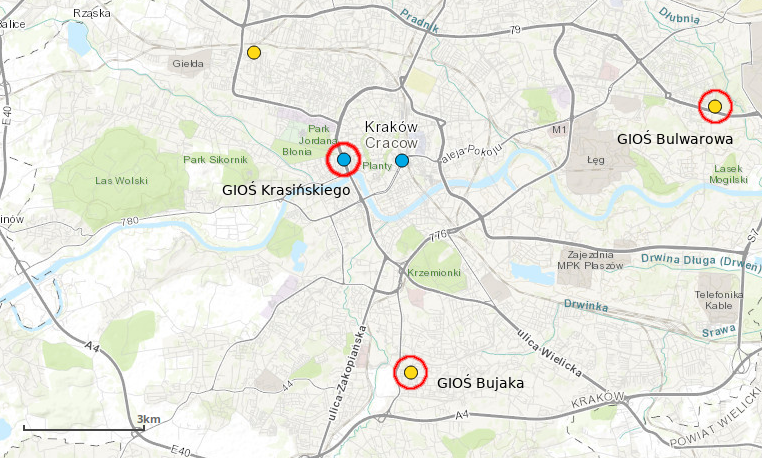
\includegraphics[scale=0.5]{figures/dataset/gios_stations.png}
\caption{Location of the air quality stations}
\label{fig:dataset-stations-location}
\end{figure}

\section{Weather factors}\label{sec:weather-data}
Air quality monitoring stations used in this study are not equipped with sensors measuring weather factors. Because of that it was decided to combine the PM2.5 measurements with meteorological data obtained from other sources: a weather station (specifically Vaisala WXT520) operated by the Faculty of Physics and Computer Science at the AGH University, sensors belonging to Airly (a local air quality monitoring company) and the Weather Underground service. The following weather variables were used in this study:
\begin{enumerate}
    \item atmospheric pressure,
    \item humidity,
    \item precipitation rate,
    \item total precipitation during the given day,
    \item temperature,
    \item wind speed,
    \item wind direction - divided into two components - North - South and East - West according to formulas \ref{eq:methodology-wind-dir-ns} and \ref{eq:methodology-wind-dir-ew}, where ${dir}_{deg}$ means wind direction expressed in degrees; directions correspond to the following angles: North - 0 $\degree$, East - 90 $\degree$, South - 180 $\degree$, West - 270 $\degree$; a visual interpretation of the variables can be seen in figure \ref{fig:dataset-wind-direction-components}.
\end{enumerate}

\begin{equation} \label{eq:methodology-wind-dir-ns}
{dir}_{North-South}({dir}_{deg}) =  sin({dir}_{deg}\frac{2 \pi}{360})
\end{equation}

\begin{equation} \label{eq:methodology-wind-dir-ew}
{dir}_{East-West}({dir}_{deg}) =  cos({dir}_{deg}\frac{2 \pi}{360})
\end{equation}
\\
\begin{figure}[htp]
    \centering
    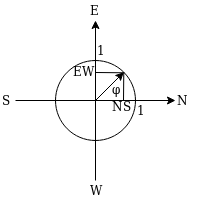
\includegraphics[scale=1]{figures/dataset/wind_direction.png}
    \caption{Wind direction components - North - South and East - West}
    \label{fig:dataset-wind-direction-components}
\end{figure}\\
Weather variables were combined with the PM2.5 concentrations based on the time of measurement and the geographical coordinates of the stations. The distances between stations were approximated by the formula \ref{eq:dataset-lat-lon-distance} based on the Spherical Law of Cosines, where $\phi$ symbolises the latitude and $\lambda$ is the longitude.

\begin{equation} \label{eq:dataset-lat-lon-distance}
dist(\phi_1, \lambda_1, \phi_2, \lambda_2) \approx acos(sin(\phi_1) sin(\phi_2) + cos(\phi_1)cos(\phi_2)cos(\lambda_2 - \lambda_1))
\end{equation}

\section{Additional variables}\label{sec:additional-variables}
The original data set was extended with a few auxiliary temporal variables intended to represent different types of seasonality, namely:
\begin{enumerate}
    \item hour of the day,
    \item period of the day - it is assumed that a 24-hour period consists of 4 parts: morning (6 a.m. - 12 p.m.), afternoon (12 p.m. - 6 p.m.), evening (6 p.m. - 12 a.m.), night (12 a.m. - 6 a.m.);
    \item day of the week,
    \item a flag indicating, whether the measurement was taken during a weekday or a weekend\,/\,a\,holiday (however, the movable holidays were not taken into consideration),
    \item month,
    \item day of the year,
    \item season - a numeric value in the range 1 - 4, where 1 represents winter, 2 - spring, 3 - summer, 4 - autumn,
    \item a flag indicating, if the measurement was taken during the heating season, which is assumed to start in September and end at the beginning of April,
    \item year.
\end{enumerate}
In the case of variables that express a fraction of a larger whole (e.g. day of the year = $\frac{day\  count}{365}$) their values were calculated as cosines of those fractions scaled and shifted in such a way, that the beginning and end of the period correspond with 0 while its centre to 1 (see equation \ref{eq:methodology-part-of-period}). Figure \ref{fig:dataset-cosine-transformation} shows the relationship between the day of the year and the value assigned to it (plots for other such variables are similar).
\\
For some variables (PM2.5 concentrations, relative humidity, precipitation rate, atmospheric pressure, temperature, wind speed and wind direction) their aggregated values (minimum, average and maximum) were also calculated for every consecutive 24 hourly measurements. Temporal variables and the cumulative daily precipitation, which is an aggregated value itself, were excluded from the process.

\begin{equation} \label{eq:methodology-part-of-period}
{Part\ of\ period}(x) = -0.5 cos(2 \pi \frac{x}{period\ length}) + 0.5
\end{equation}

\begin{figure}[htp]
\centering
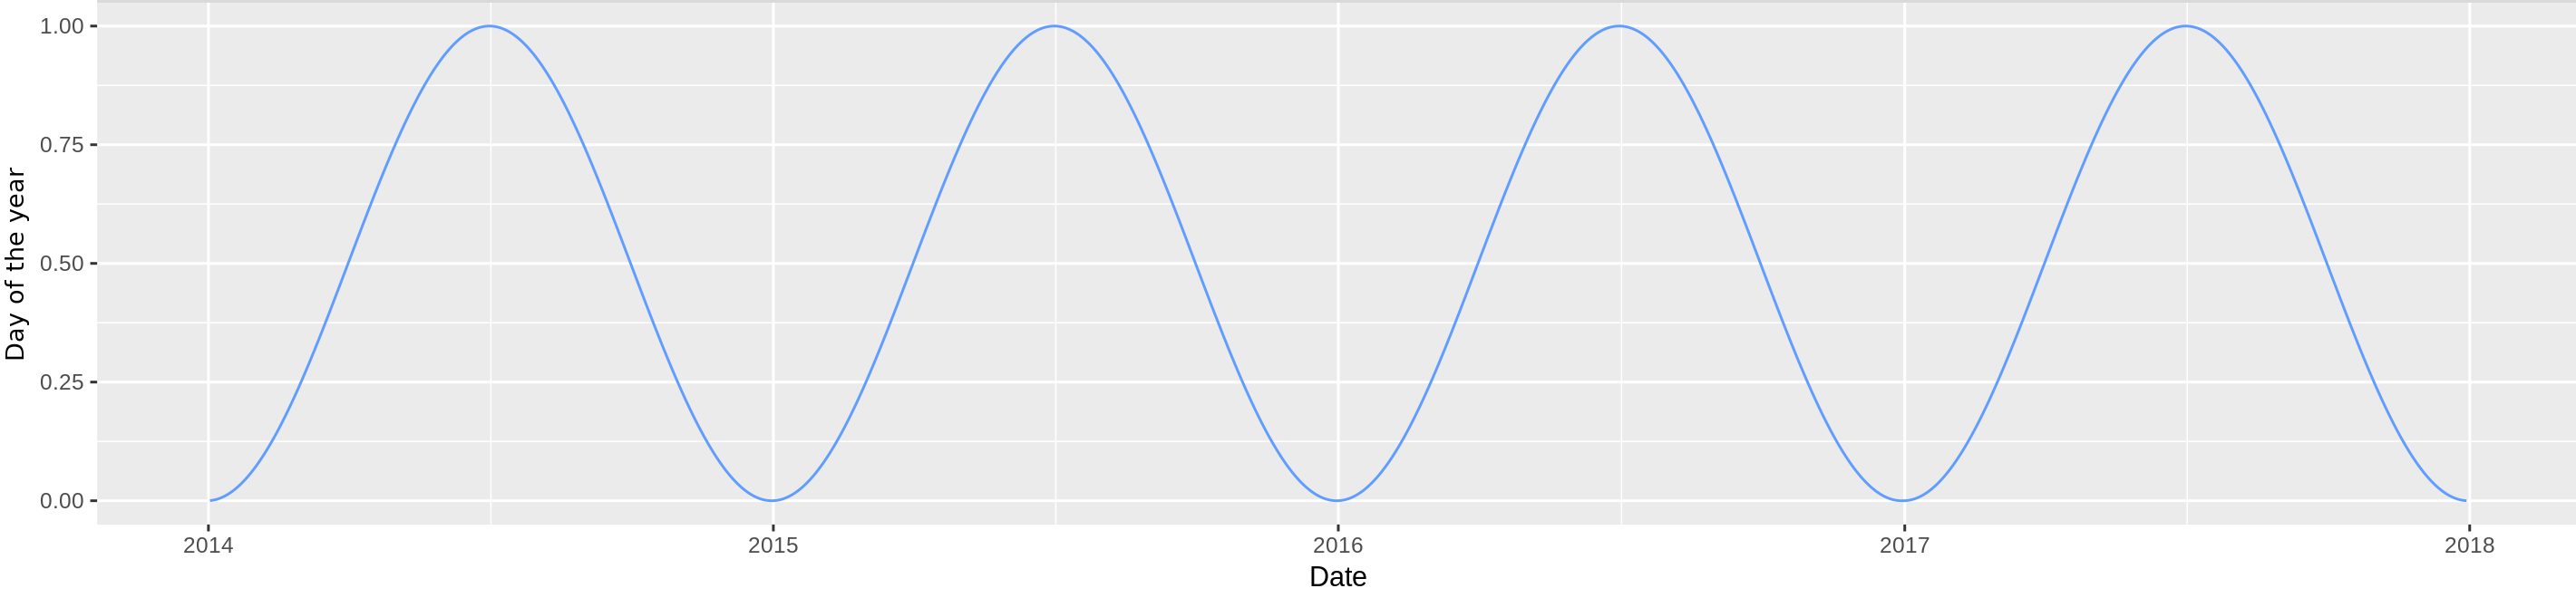
\includegraphics[width=\textwidth]{figures/dataset/fraction_of_period.png}
\caption{Result of the cosine transformation - day of the year}
\label{fig:dataset-cosine-transformation}
\end{figure}


\section{Anomaly detection}
The data set was tested for existence of measurements (\textit{outliers}) that do not match other observations registered in similar conditions. The process of eliminating them consisted of two steps:
\begin{enumerate}
    \item filtering out observations with values too extreme for climate that Krakow is located in - chosen thresholds are presented in table \ref{tab:dataset-anomaly-thresholds},
    \item analysis of histograms of each variable prepared for specific month and year and removing values that are relatively large/small and, at the same time, more frequent than the neighbouring ones.
\end{enumerate}

\begin{table}[H]
\centering
\caption{Thresholds used for anomaly detection}
\label{tab:dataset-anomaly-thresholds}
\begin{tabular}{llrr}
\toprule
Variable               & Units       & Lower threshold & Upper threshold \\ \midrule
Air humidity           & $\%$        & 0               & 100             \\
Air pressure           & $hPa$       & 970             & 1050            \\
Precipitation rate/sum & $mm$        & 0               & -               \\
Temperature            & $\degree C$ & -25             & 40              \\ 
Wind direction         & $\degree$   & 0               & 360             \\
Wind speed             & $m/s$       & 0               & -               \\ 
\bottomrule
\end{tabular}
\end{table}

\section{Missing data}
The air quality data were found to be incomplete with the number of missing PM2.5 concentrations ranging from 1.65\% to 3.27\%, depending on the station (table \ref{tab:dataset-missing-pm25}). Missing values were approximated using the Multiple Imputation by Chained Equations method \cite{MICE2011}, which is based on the idea of estimating the distribution of a specific variable based on the available data and drawing samples from that distribution (\textit{Gibbs sampling}). The decision of applying an imputation method instead of simply omitting the lacking records was taken in order to make the data set suitable for models that require the time series to be continuous e.g. ARIMA.

\begin{table}[H]
\centering
\caption{Percentage of missing PM2.5 measurements per station}
\label{tab:dataset-missing-pm25}
\begin{tabular}{lr}
\toprule
Station           & Missing PM2.5 {[}\%{]} \\ \midrule
GIOŚ Bujaka       & 2.920                  \\
GIOŚ Bulwarowa    & 3.271                  \\
GIOŚ Krasińskiego & 1.648                  \\ \bottomrule
\end{tabular}
\end{table}

\section{Data statistics}
After finishing the preprocessing steps, monthly means and standard deviations were calculated for the main variables used in this study: PM2.5, air humidity, total precipitation, air pressure, temperature, wind direction and speed. Results are presented in tables \ref{tab:dataset-stats-bujaka} - \ref{tab:dataset-stats-krasinskiego}, separately for each station.
\\\\
Figures \ref{fig:dataset-trend-pm25} - \ref{fig:dataset-trend-wind-speed} depict daily mean values of the variables. Some of them display strong seasonality: PM2.5 levels are highest in winter and lowest during summer, while temperatures and daily total precipitation show the opposite behaviour: they are highest during summer and lowest in winter. Humidity levels peak in autumn and reach lowest values during summer. 
\\\\
In the case of pressure, wind direction and speed one can notice that mean values increase with time, for example: pressure measured by stations Bujaka and Krasińskiego in 2014 tends to reach lower levels than in 2017. It is probably caused by mixing measurements from different sources in the case of activating a new weather sensor located closer to the air quality station.
\\\\
Scatter plots \ref{fig:dataset-bivariate-bujaka} - \ref{fig:dataset-bivariate-krasinskiego} depict relationships between the concentrations of PM2.5 at the moment T + 24 hours and the main explanatory variables mentioned in the previous paragraphs. They seem to be similar for all of the monitoring stations. Wind speed, total precipitation and, to some extent, temperature and humidity, display fairly strong nonlinear relationships with future PM2.5 levels. Dispersion of the PM2.5 concentrations for the same value of the predictor might be significant, however their maximum levels seem to be limited by nonlinear functions of the weather factors. PM2.5 concentrations, on the other hand, show a weak linear dependency on future PM2.5 levels - points on the scatter plots form cones, rather than lines. In the case of wind direction the widest range of PM2.5 levels corresponds roughly to 90$\degree$ and 270$\degree$, which is probably indicative of the fact that in Krakow West and East winds are the most common. 
\\\\
Table \ref{tab:dataset-correlation-significant} contains a ranking of the variables ordered by the corresponding absolute value of the Pearson correlation coefficient. The comparison was prepared separately for each of the monitoring stations and seasons. In each case the first position on the list is occupied by PM2.5 concentrations, while next variables vary, depending on the season. For winter they are: temperature, pressure and wind speed, for spring: day of the year, month, heating season, temperature and the period of the day, for summer: wind speed, day of year, pressure and month and for autumn: wind speed, pressure, temperature, day of the year and month.
\begin{landscape}
\begin{table}[H]
\centering
\caption{Variable statistics - GIOŚ Bujaka}
\label{tab:dataset-stats-bujaka}
\footnotesize
\begin{tabular}{llrrrrrrrrrrrrr}
\hline
Month & \multicolumn{2}{c}{PM2.5} & \multicolumn{2}{c}{Humidity} & \multicolumn{2}{c}{Total precipitation} & \multicolumn{2}{c}{Pressure} & \multicolumn{2}{c}{Temperature} & \multicolumn{2}{c}{Wind direction} & \multicolumn{2}{c}{Wind speed} \\
Units & \multicolumn{2}{c}{$\mu g / m^3$} & \multicolumn{2}{c}{$\%$} & \multicolumn{2}{c}{$mm$} & \multicolumn{2}{c}{$hPa$} & \multicolumn{2}{c}{$\degree C$} & \multicolumn{2}{c}{$\degree$} & \multicolumn{2}{c}{$m/s$} \\
Type & mean & std & mean & std & mean & std & mean & std & mean & std & mean & std & mean & std \\ \hline
January & 66.15 & 65.510 & 71.31 & 15.25 & 0.2052 & 0.7041 & 1004 & 17.38 & -0.5669 & 5.655 & 197.2 & 80.85 & 1.784 & 1.575 \\
February & 54.88 & 49.481 & 74.73 & 14.45 & 0.3133 & 1.0124 & 1007 & 15.34 & 3.1434 & 4.474 & 204.0 & 76.31 & 1.612 & 1.707 \\
March & 39.36 & 37.173 & 67.76 & 18.24 & 0.4025 & 1.3471 & 1009 & 14.74 & 6.5556 & 4.403 & 196.1 & 82.74 & 1.907 & 1.677 \\
April & 23.19 & 17.813 & 64.06 & 18.76 & 0.7157 & 2.2453 & 1007 & 13.33 & 10.1336 & 5.850 & 212.6 & 74.19 & 1.922 & 1.556 \\
May & 16.22 & 9.709 & 68.09 & 19.16 & 0.8329 & 2.3249 & 1007 & 13.36 & 14.9760 & 5.193 & 199.3 & 78.65 & 1.614 & 1.261 \\
June & 13.84 & 8.355 & 60.63 & 17.74 & 1.0023 & 3.9264 & 1008 & 11.70 & 19.1260 & 5.282 & 210.3 & 71.78 & 1.756 & 1.468 \\
July & 11.13 & 6.721 & 63.03 & 18.90 & 1.2676 & 4.4290 & 1007 & 12.85 & 21.0025 & 5.316 & 214.9 & 70.83 & 1.681 & 1.427 \\
August & 15.13 & 9.839 & 63.30 & 18.45 & 1.1871 & 5.9126 & 1009 & 14.08 & 20.2478 & 5.766 & 205.9 & 72.24 & 1.345 & 1.108 \\
September & 16.81 & 11.083 & 72.49 & 17.36 & 1.2302 & 3.9272 & 1009 & 12.65 & 15.6200 & 5.529 & 195.0 & 79.44 & 1.516 & 1.302 \\
October & 30.30 & 25.019 & 77.46 & 13.06 & 0.8068 & 2.7478 & 1010 & 13.60 & 9.3803 & 4.633 & 196.1 & 77.04 & 1.537 & 1.753 \\
November & 41.13 & 38.661 & 77.88 & 11.34 & 0.5977 & 1.4971 & 1009 & 13.12 & 5.7905 & 4.535 & 204.7 & 70.16 & 1.373 & 1.590 \\
December & 42.92 & 41.027 & 74.92 & 14.16 & 0.3207 & 1.1101 & 1013 & 15.80 & 2.8558 & 4.422 & 220.8 & 60.25 & 2.344 & 2.493 \\ \hline
\end{tabular}
\end{table}
\end{landscape}

\begin{landscape}
\begin{table}[H]
\centering
\caption{Variable statistics - GIOŚ Bulwarowa}
\label{tab:dataset-stats-bulwarowa}
\footnotesize
\begin{tabular}{llrrrrrrrrrrrrr}
\hline
Month & \multicolumn{2}{c}{PM2.5} & \multicolumn{2}{c}{Humidity} & \multicolumn{2}{c}{Total precipitation} & \multicolumn{2}{c}{Pressure} & \multicolumn{2}{c}{Temperature} & \multicolumn{2}{c}{Wind direction} & \multicolumn{2}{c}{Wind speed} \\
Units & \multicolumn{2}{c}{$\mu g / m^3$} & \multicolumn{2}{c}{$\%$} & \multicolumn{2}{c}{$mm$} & \multicolumn{2}{c}{$hPa$} & \multicolumn{2}{c}{$\degree C$} & \multicolumn{2}{c}{$\degree$} & \multicolumn{2}{c}{$m/s$} \\
Type & mean & std & mean & std & mean & std & mean & std & mean & std & mean & std & mean & std \\ \hline

January & 57.97 & 51.12 & 69.52 & 25.12 & 0.36 & 0.92 & 1013.37 & 12.26 & 0.09 & 5.20 & 203.32 & 110.84 & 3.31 & 4.39 \\ 
February & 51.42 & 40.53 & 75.13 & 13.81 & 0.76 & 1.98 & 1014.18 & 10.20 & 3.32 & 4.15 & 191.45 & 117.19 & 2.32 & 3.37 \\ 
March & 38.41 & 30.73 & 69.52 & 16.96 & 0.67 & 1.86 & 1015.63 & 9.88 & 6.85 & 4.37 & 217.33 & 111.75 & 3.48 & 4.43 \\ 
April & 23.87 & 16.83 & 65.81 & 18.79 & 0.87 & 2.55 & 1013.73 & 6.30 & 10.43 & 5.63 & 229.04 & 92.69 & 3.47 & 4.22 \\ 
May & 17.81 & 11.30 & 67.64 & 18.66 & 1.15 & 3.35 & 1013.64 & 5.93 & 15.51 & 5.22 & 219.83 & 63.23 & 2.39 & 3.66 \\ 
June & 13.92 & 8.91 & 60.19 & 18.50 & 0.99 & 4.03 & 1014.39 & 5.50 & 19.62 & 5.39 & 227.61 & 57.52 & 1.64 & 2.32 \\ 
July & 13.09 & 7.67 & 64.69 & 18.77 & 1.33 & 3.98 & 1013.65 & 4.73 & 21.32 & 5.26 & 249.09 & 70.67 & 2.03 & 2.94 \\ 
August & 17.00 & 10.94 & 66.50 & 18.53 & 1.34 & 6.37 & 1016.08 & 4.00 & 20.79 & 5.89 & 256.25 & 69.42 & 1.15 & 1.79 \\ 
September & 19.12 & 12.50 & 74.88 & 15.88 & 1.31 & 4.15 & 1016.34 & 6.14 & 15.86 & 5.27 & 223.47 & 89.16 & 1.75 & 2.88 \\ 
October & 32.31 & 24.79 & 80.81 & 12.58 & 1.20 & 3.98 & 1018.17 & 6.87 & 9.65 & 4.58 & 213.50 & 93.90 & 2.48 & 5.29 \\ 
November & 43.56 & 38.29 & 82.70 & 10.50 & 0.71 & 1.69 & 1015.76 & 8.06 & 5.73 & 4.45 & 196.89 & 103.70 & 4.30 & 5.42 \\ 
December & 41.36 & 35.74 & 81.19 & 10.36 & 0.26 & 0.79 & 1020.75 & 9.67 & 2.79 & 4.23 & 241.93 & 88.31 & 5.77 & 6.94 \\ 
\bottomrule

\end{tabular}
\end{table}
\end{landscape}


\begin{landscape}
\begin{table}[H]
\centering
\caption{Variable statistics - GIOŚ Krasińskiego}
\label{tab:dataset-stats-krasinskiego}
\footnotesize
\begin{tabular}{llrrrrrrrrrrrrr}
\hline
Month & \multicolumn{2}{c}{PM2.5} & \multicolumn{2}{c}{Humidity} & \multicolumn{2}{c}{Total precipitation} & \multicolumn{2}{c}{Pressure} & \multicolumn{2}{c}{Temperature} & \multicolumn{2}{c}{Wind direction} & \multicolumn{2}{c}{Wind speed} \\
Units & \multicolumn{2}{c}{$\mu g / m^3$} & \multicolumn{2}{c}{$\%$} & \multicolumn{2}{c}{$mm$} & \multicolumn{2}{c}{$hPa$} & \multicolumn{2}{c}{$\degree C$} & \multicolumn{2}{c}{$\degree$} & \multicolumn{2}{c}{$m/s$} \\
Type & mean & std & mean & std & mean & std & mean & std & mean & std & mean & std & mean & std \\ \hline

January & 74.02 & 59.89 & 70.23 & 14.00 & 0.19 & 0.66 & 1003.02 & 18.43 & -0.12 & 5.31 & 185.90 & 86.92 & 2.76 & 2.28 \\ 
February & 67.75 & 47.65 & 73.16 & 14.41 & 0.26 & 0.81 & 1001.84 & 16.56 & 3.05 & 4.27 & 185.54 & 85.95 & 2.84 & 2.90 \\ 
March & 48.70 & 35.66 & 66.84 & 17.49 & 0.23 & 0.89 & 1002.43 & 14.58 & 6.44 & 4.35 & 189.08 & 87.86 & 2.91 & 2.51 \\ 
April & 33.18 & 20.50 & 64.50 & 18.99 & 0.35 & 1.40 & 1000.77 & 14.18 & 9.87 & 5.56 & 207.02 & 84.75 & 3.00 & 2.80 \\ 
May & 25.59 & 13.37 & 67.48 & 18.77 & 0.74 & 2.21 & 1001.47 & 14.54 & 14.96 & 5.62 & 188.57 & 90.29 & 2.65 & 2.24 \\ 
June & 19.89 & 10.20 & 62.02 & 18.21 & 0.89 & 3.89 & 1003.25 & 13.50 & 18.87 & 5.41 & 207.62 & 80.69 & 2.63 & 2.32 \\ 
July & 20.62 & 9.25 & 65.34 & 19.55 & 1.09 & 4.33 & 1001.32 & 13.89 & 20.66 & 5.23 & 214.11 & 76.03 & 2.34 & 2.01 \\ 
August & 23.91 & 12.44 & 65.54 & 19.48 & 1.01 & 4.40 & 1003.94 & 15.15 & 20.44 & 6.02 & 197.36 & 82.27 & 2.15 & 1.83 \\ 
September & 29.00 & 14.12 & 74.22 & 17.07 & 0.72 & 2.19 & 1004.31 & 14.55 & 15.35 & 5.48 & 184.36 & 89.38 & 2.50 & 2.40 \\ 
October & 44.48 & 28.44 & 82.15 & 15.04 & 0.46 & 1.71 & 1005.63 & 14.06 & 8.96 & 4.62 & 179.76 & 86.95 & 2.55 & 2.69 \\ 
November & 58.54 & 42.27 & 81.85 & 13.53 & 0.32 & 1.06 & 1003.05 & 14.13 & 5.22 & 4.61 & 170.22 & 88.59 & 2.76 & 2.49 \\ 
December & 55.06 & 41.28 & 79.23 & 14.12 & 0.13 & 0.41 & 1007.78 & 15.57 & 2.31 & 4.48 & 214.18 & 72.72 & 4.13 & 3.43 \\ 
\bottomrule

\end{tabular}
\end{table}
\end{landscape}

% Yearly trends %

\begin{landscape}
\begin{figure}[htp]
\centering
  \centering
  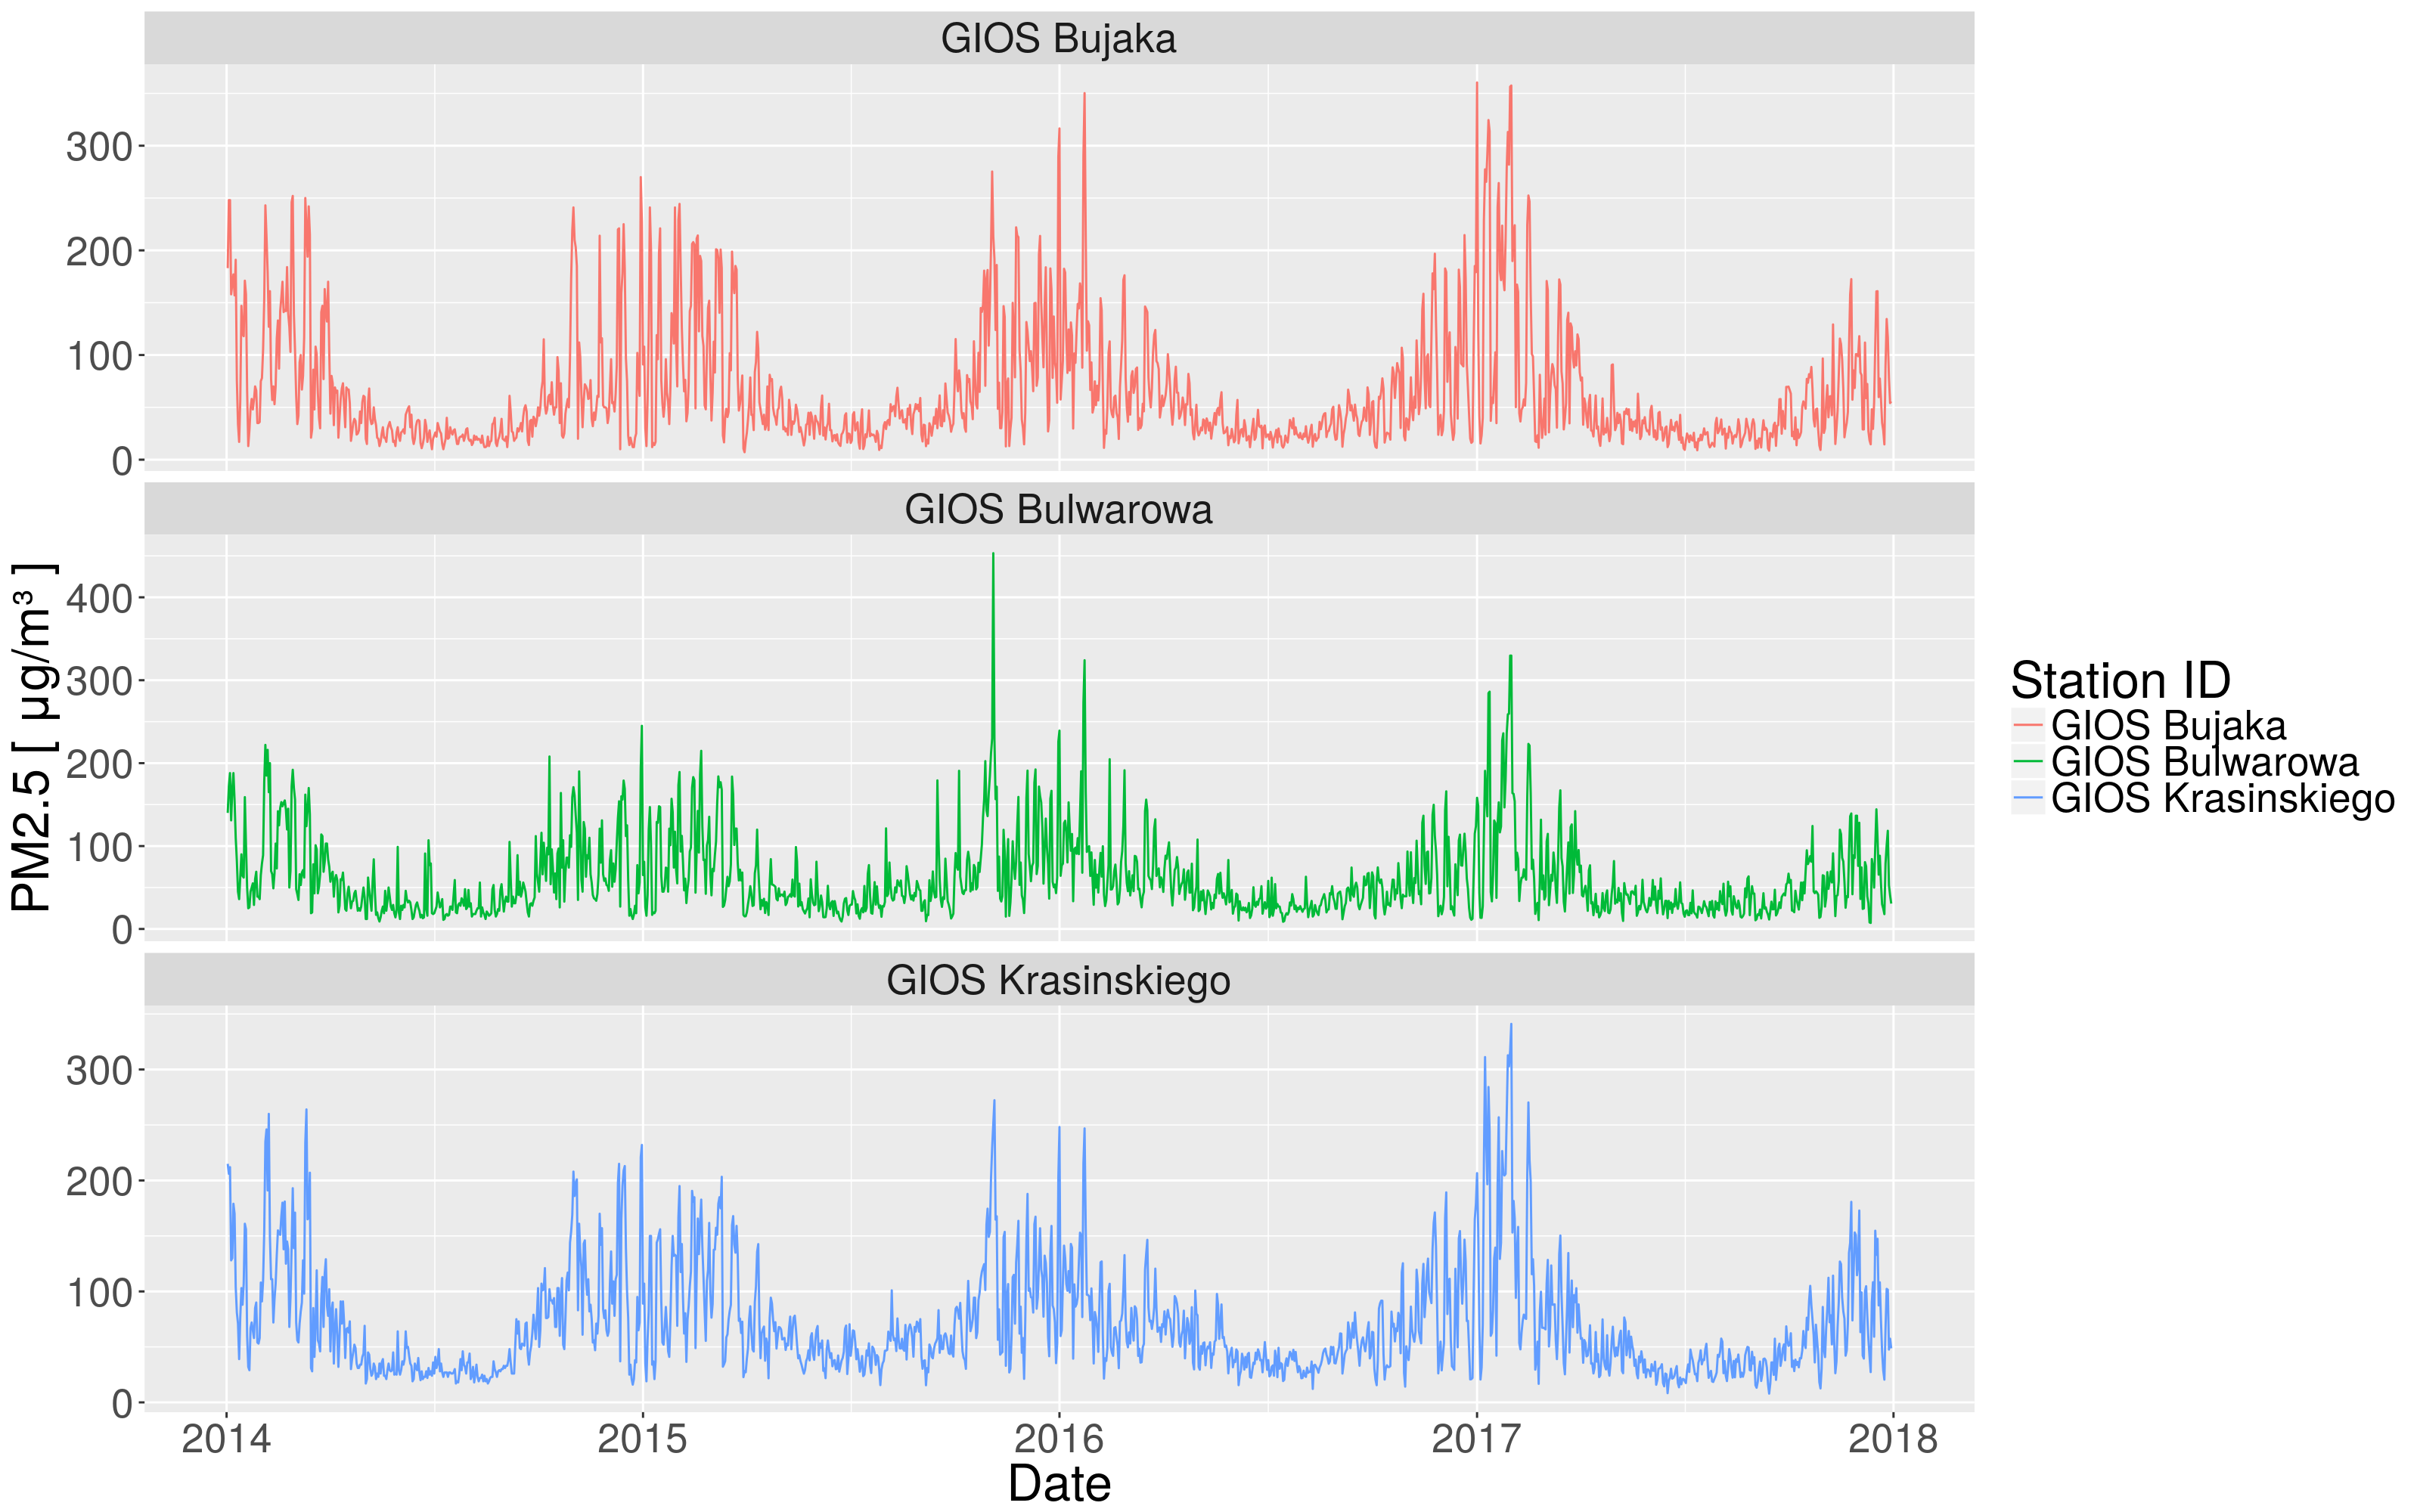
\includegraphics[width=\linewidth]{figures/dataset/trend/pm2_5_yearly_trend.png}
  \caption{Mean daily PM2.5 concentrations}
  \label{fig:dataset-trend-pm25}
\end{figure}
\end{landscape}
\begin{landscape}
\begin{figure}[htp]
\centering
  \centering
  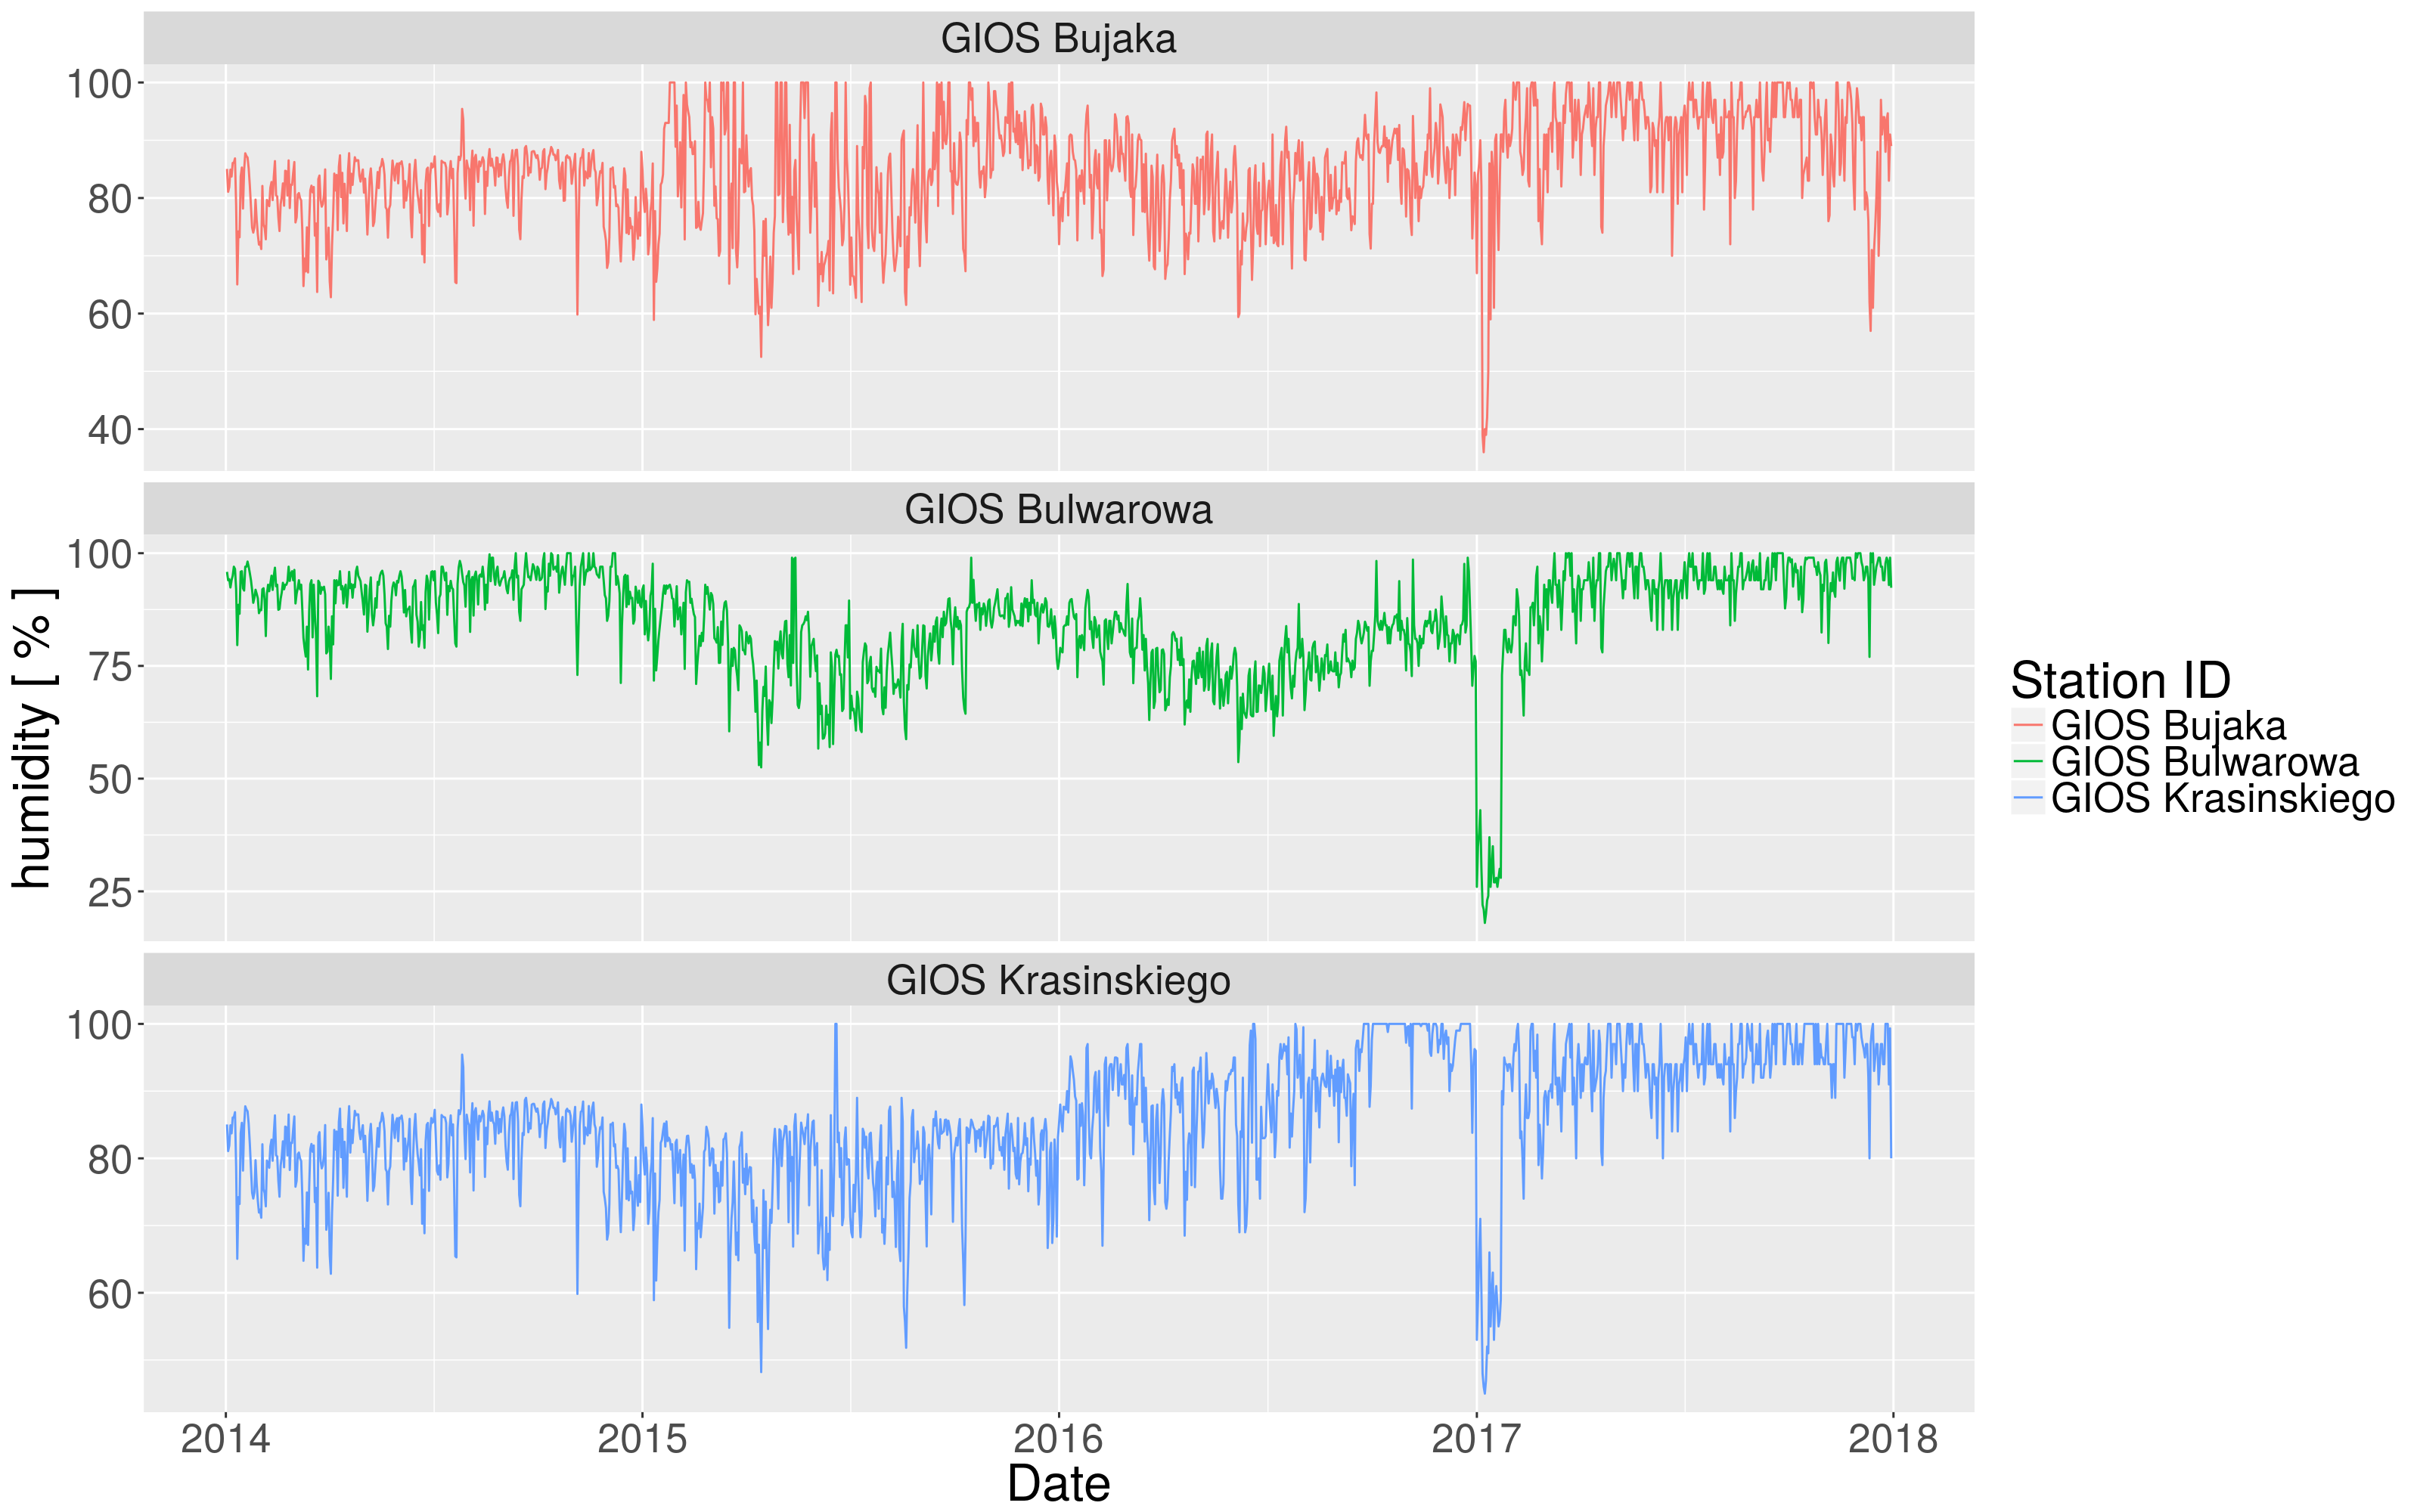
\includegraphics[width=\linewidth]{figures/dataset/trend/humidity_yearly_trend.png}
  \caption{Mean daily humidity}
  \label{fig:dataset-trend-humidity}
\end{figure}
\end{landscape}
\begin{landscape}
\begin{figure}[htp]
\centering
  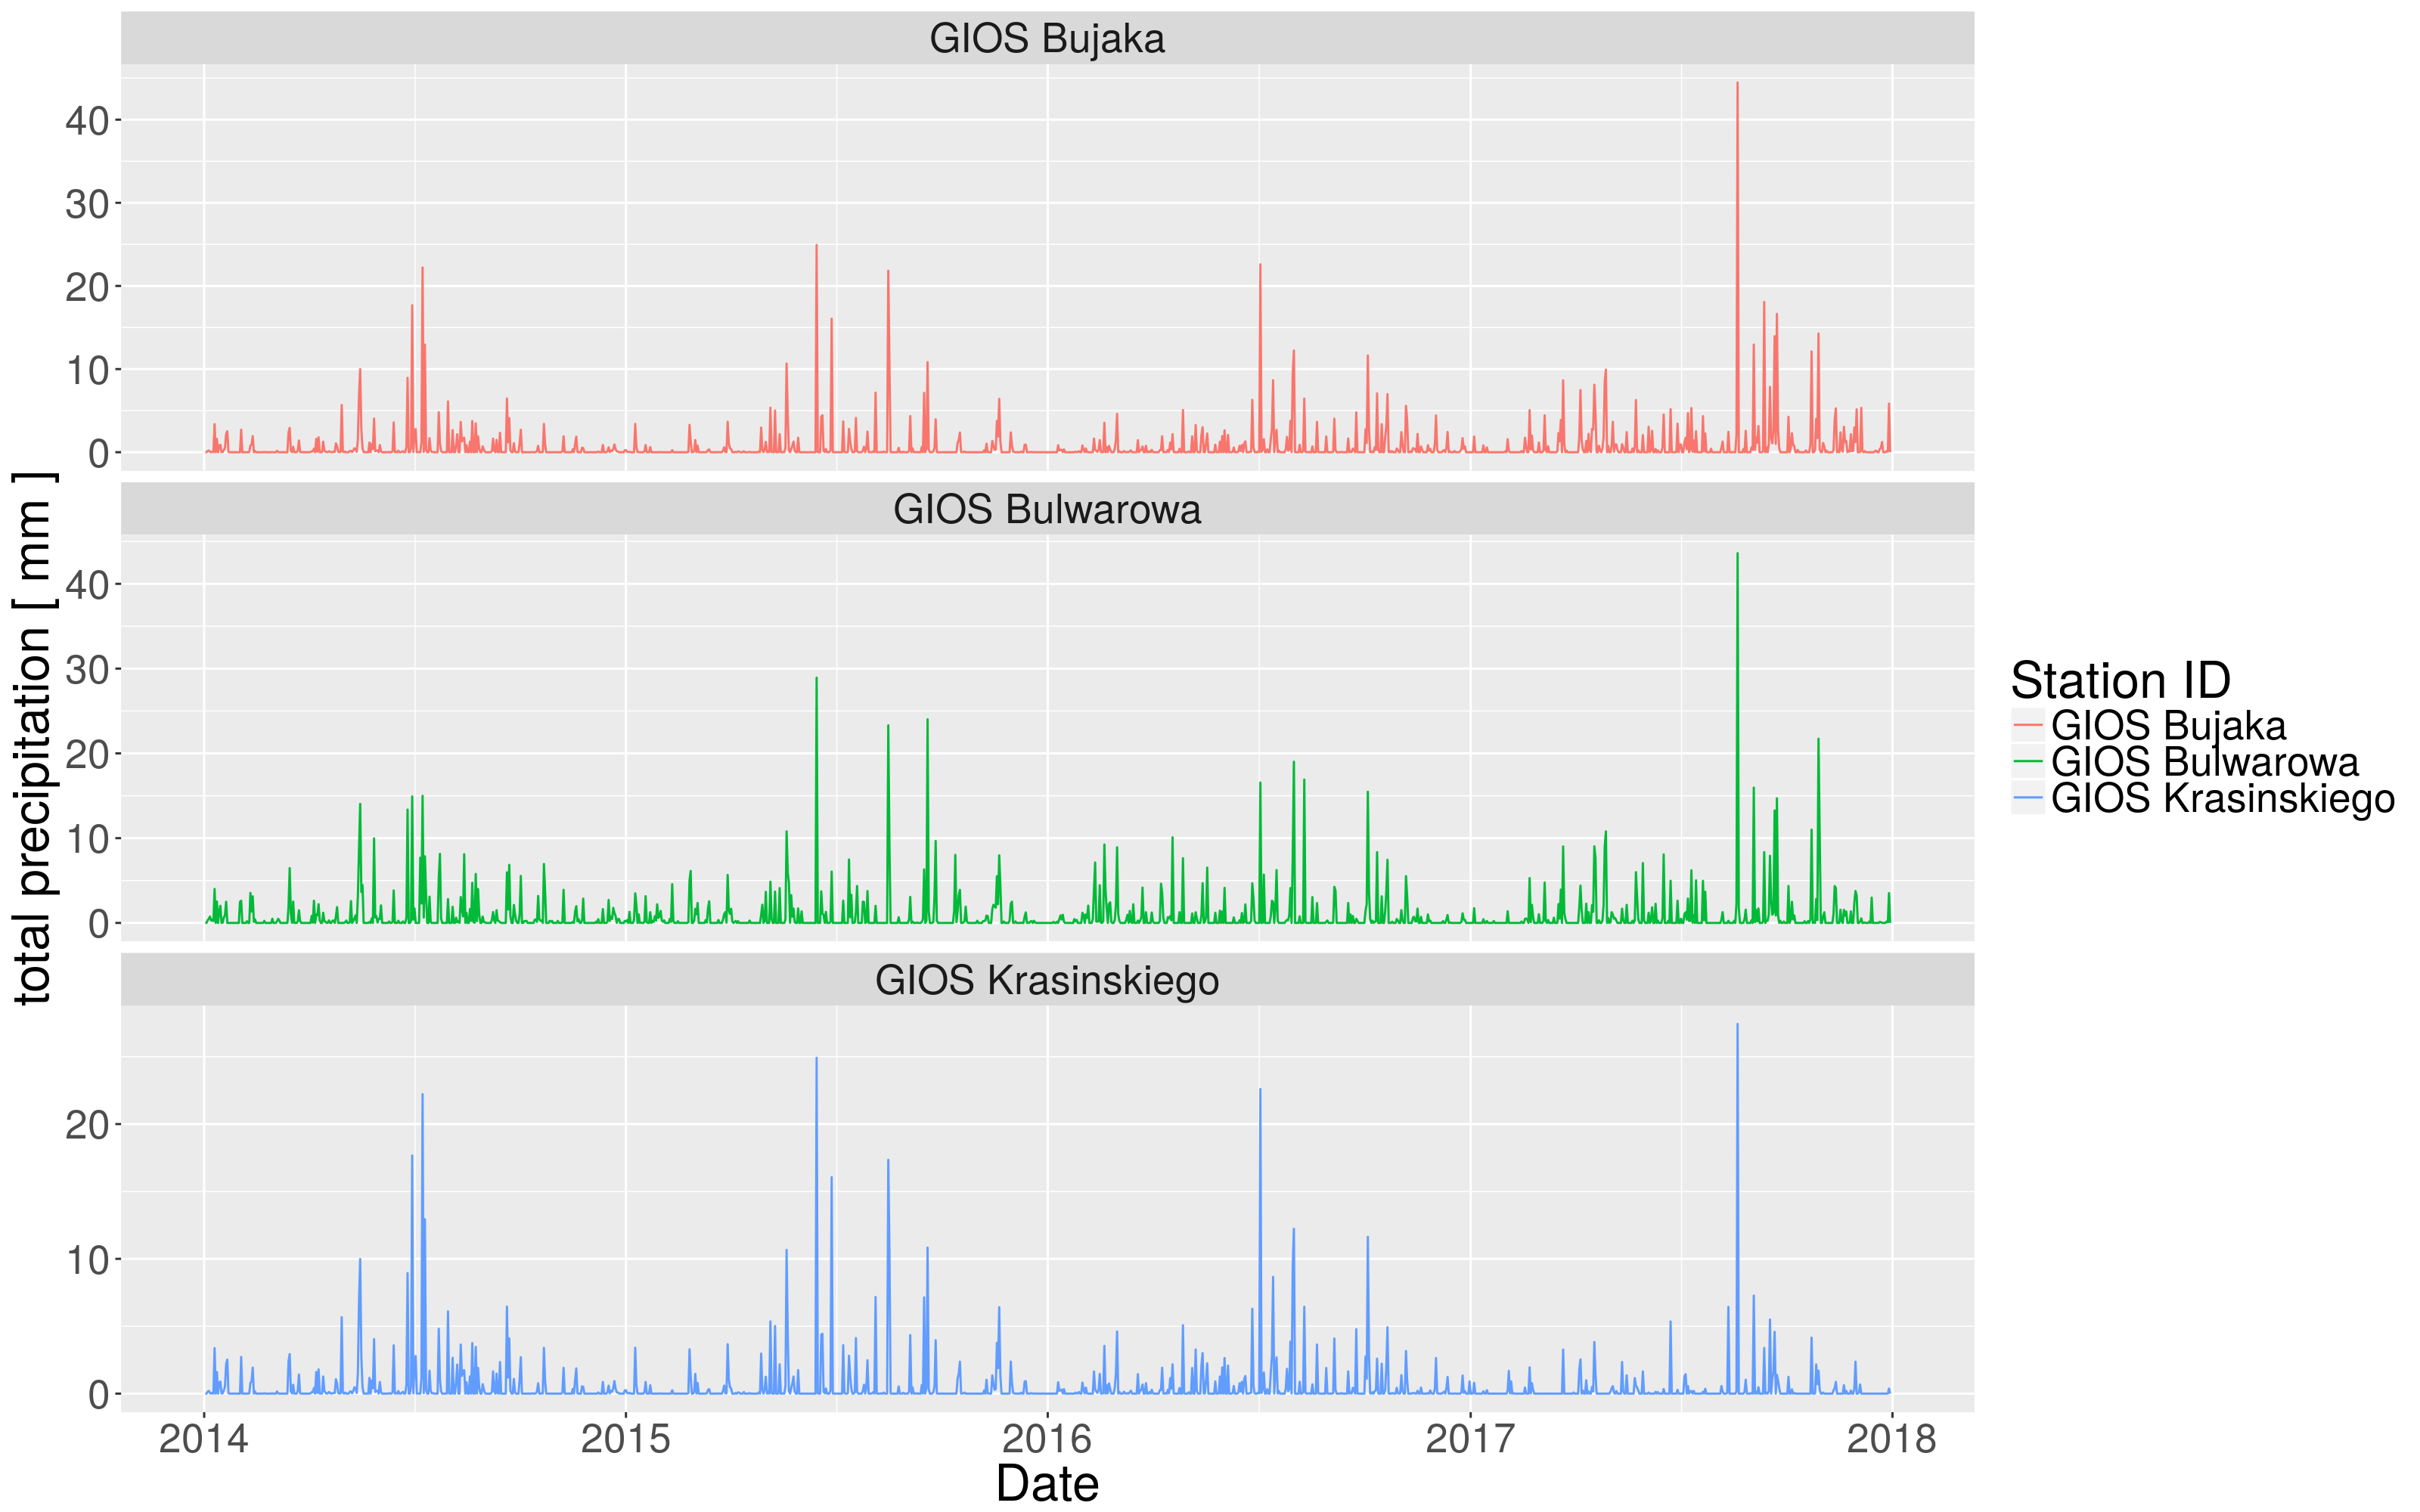
\includegraphics[width=\linewidth]{figures/dataset/trend/precip_total_yearly_trend.png}
  \caption{Daily total precipitation}
  \label{fig:dataset-trend-precip-total}
\end{figure}
\end{landscape}
\begin{landscape}
\begin{figure}[htp]
\centering
  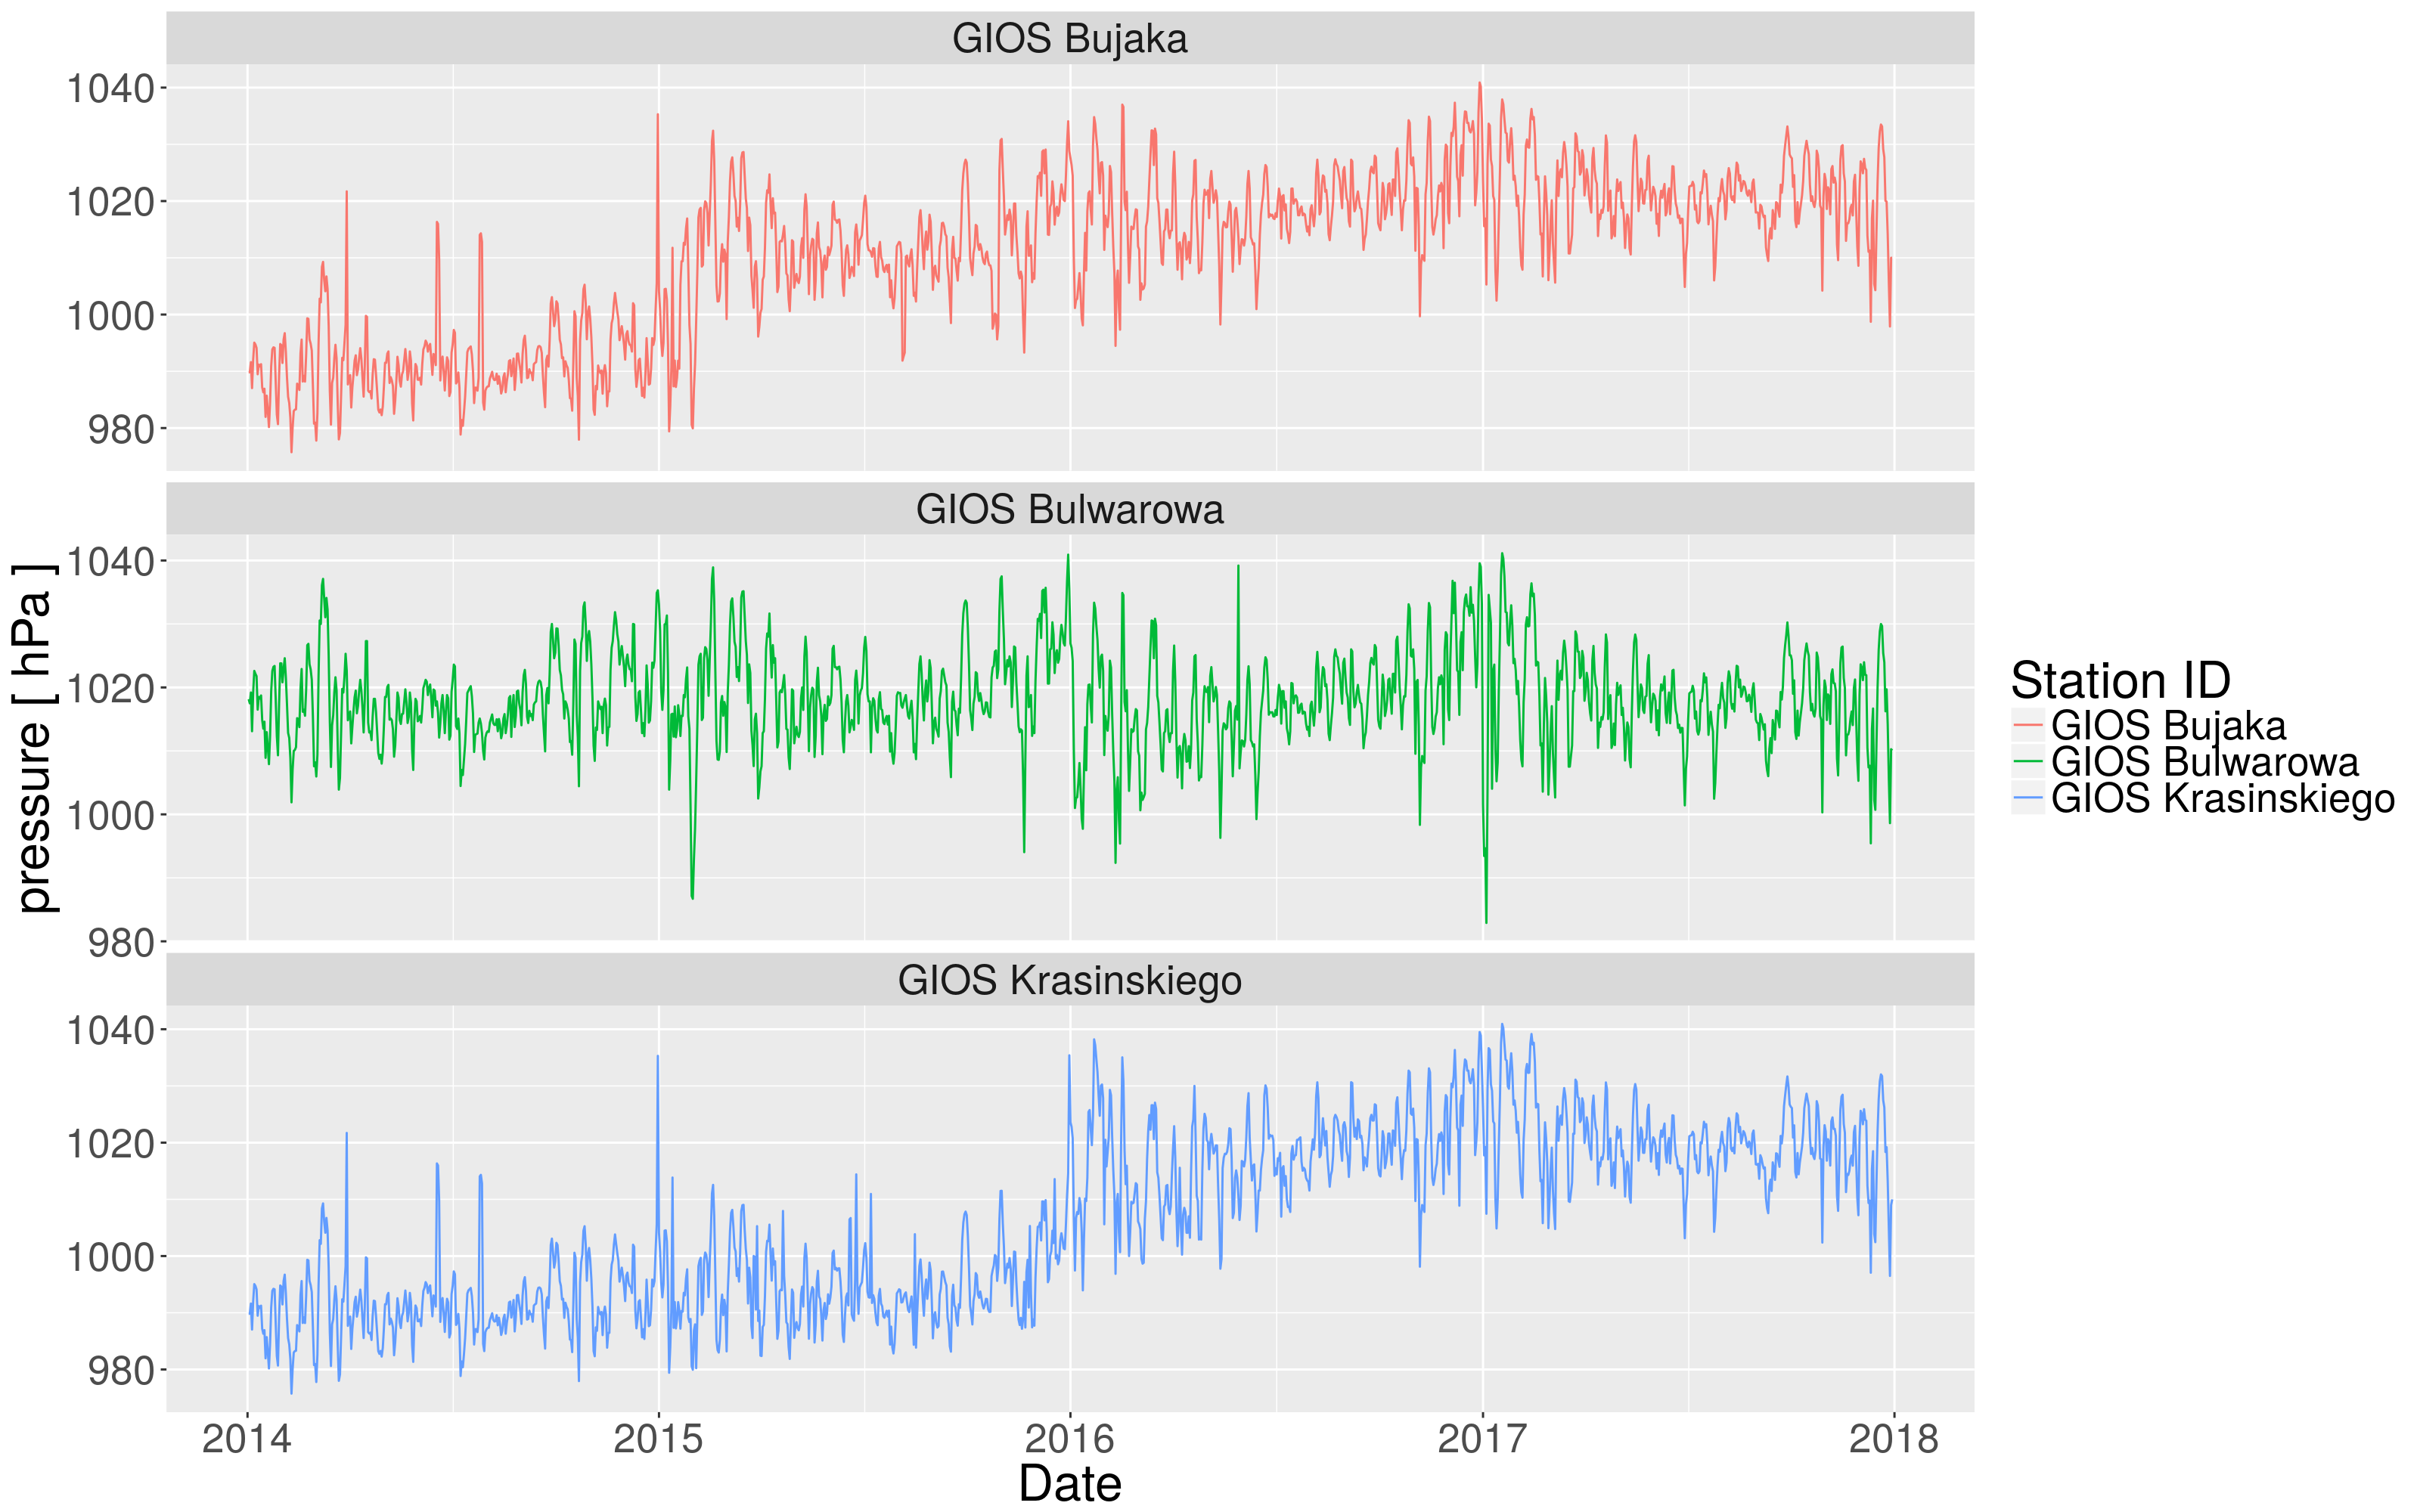
\includegraphics[width=\linewidth]{figures/dataset/trend/pressure_yearly_trend.png}
  \caption{Mean daily atmospheric pressure}
  \label{fig:dataset-trend-pressure}
\end{figure}
\end{landscape}
\begin{landscape}
\begin{figure}[htp]
\centering
  \centering
      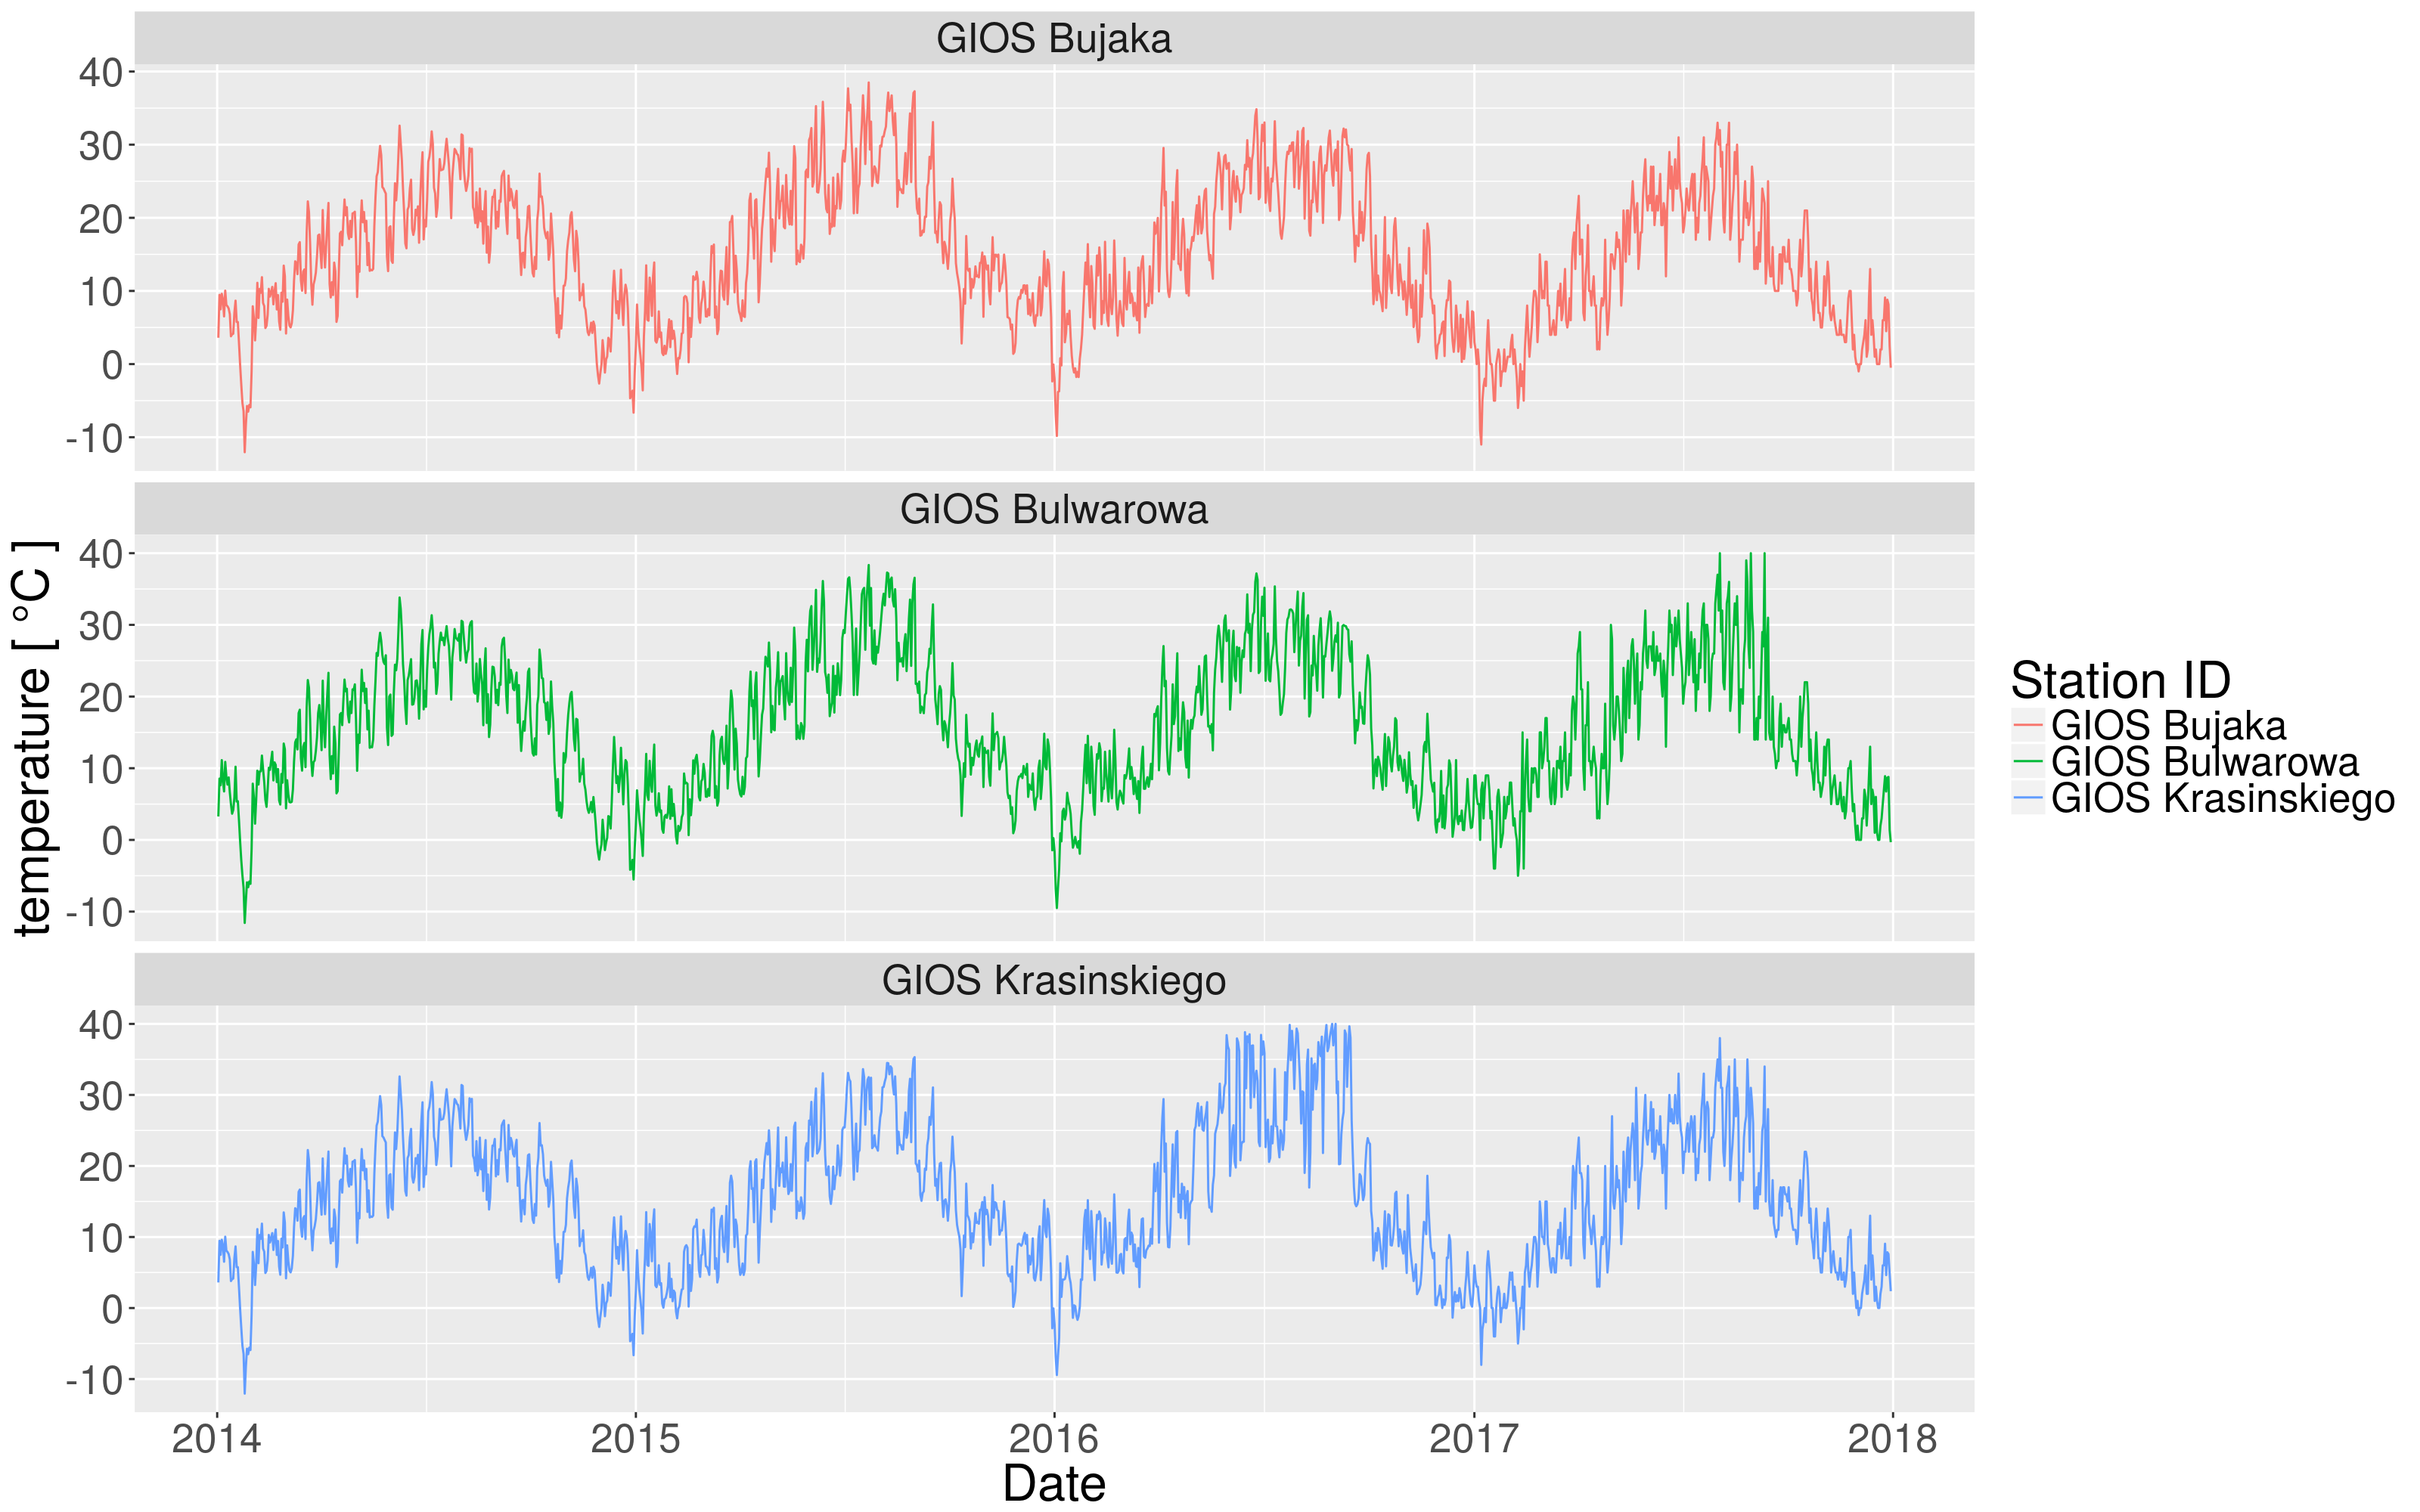
\includegraphics[width=\linewidth]{figures/dataset/trend/temperature_yearly_trend.png}
  \caption{Mean daily temperature}
  \label{fig:dataset-trend-temperature}
\end{figure}
\end{landscape}

\begin{landscape}
\begin{figure}[htp]
\centering
  \centering
  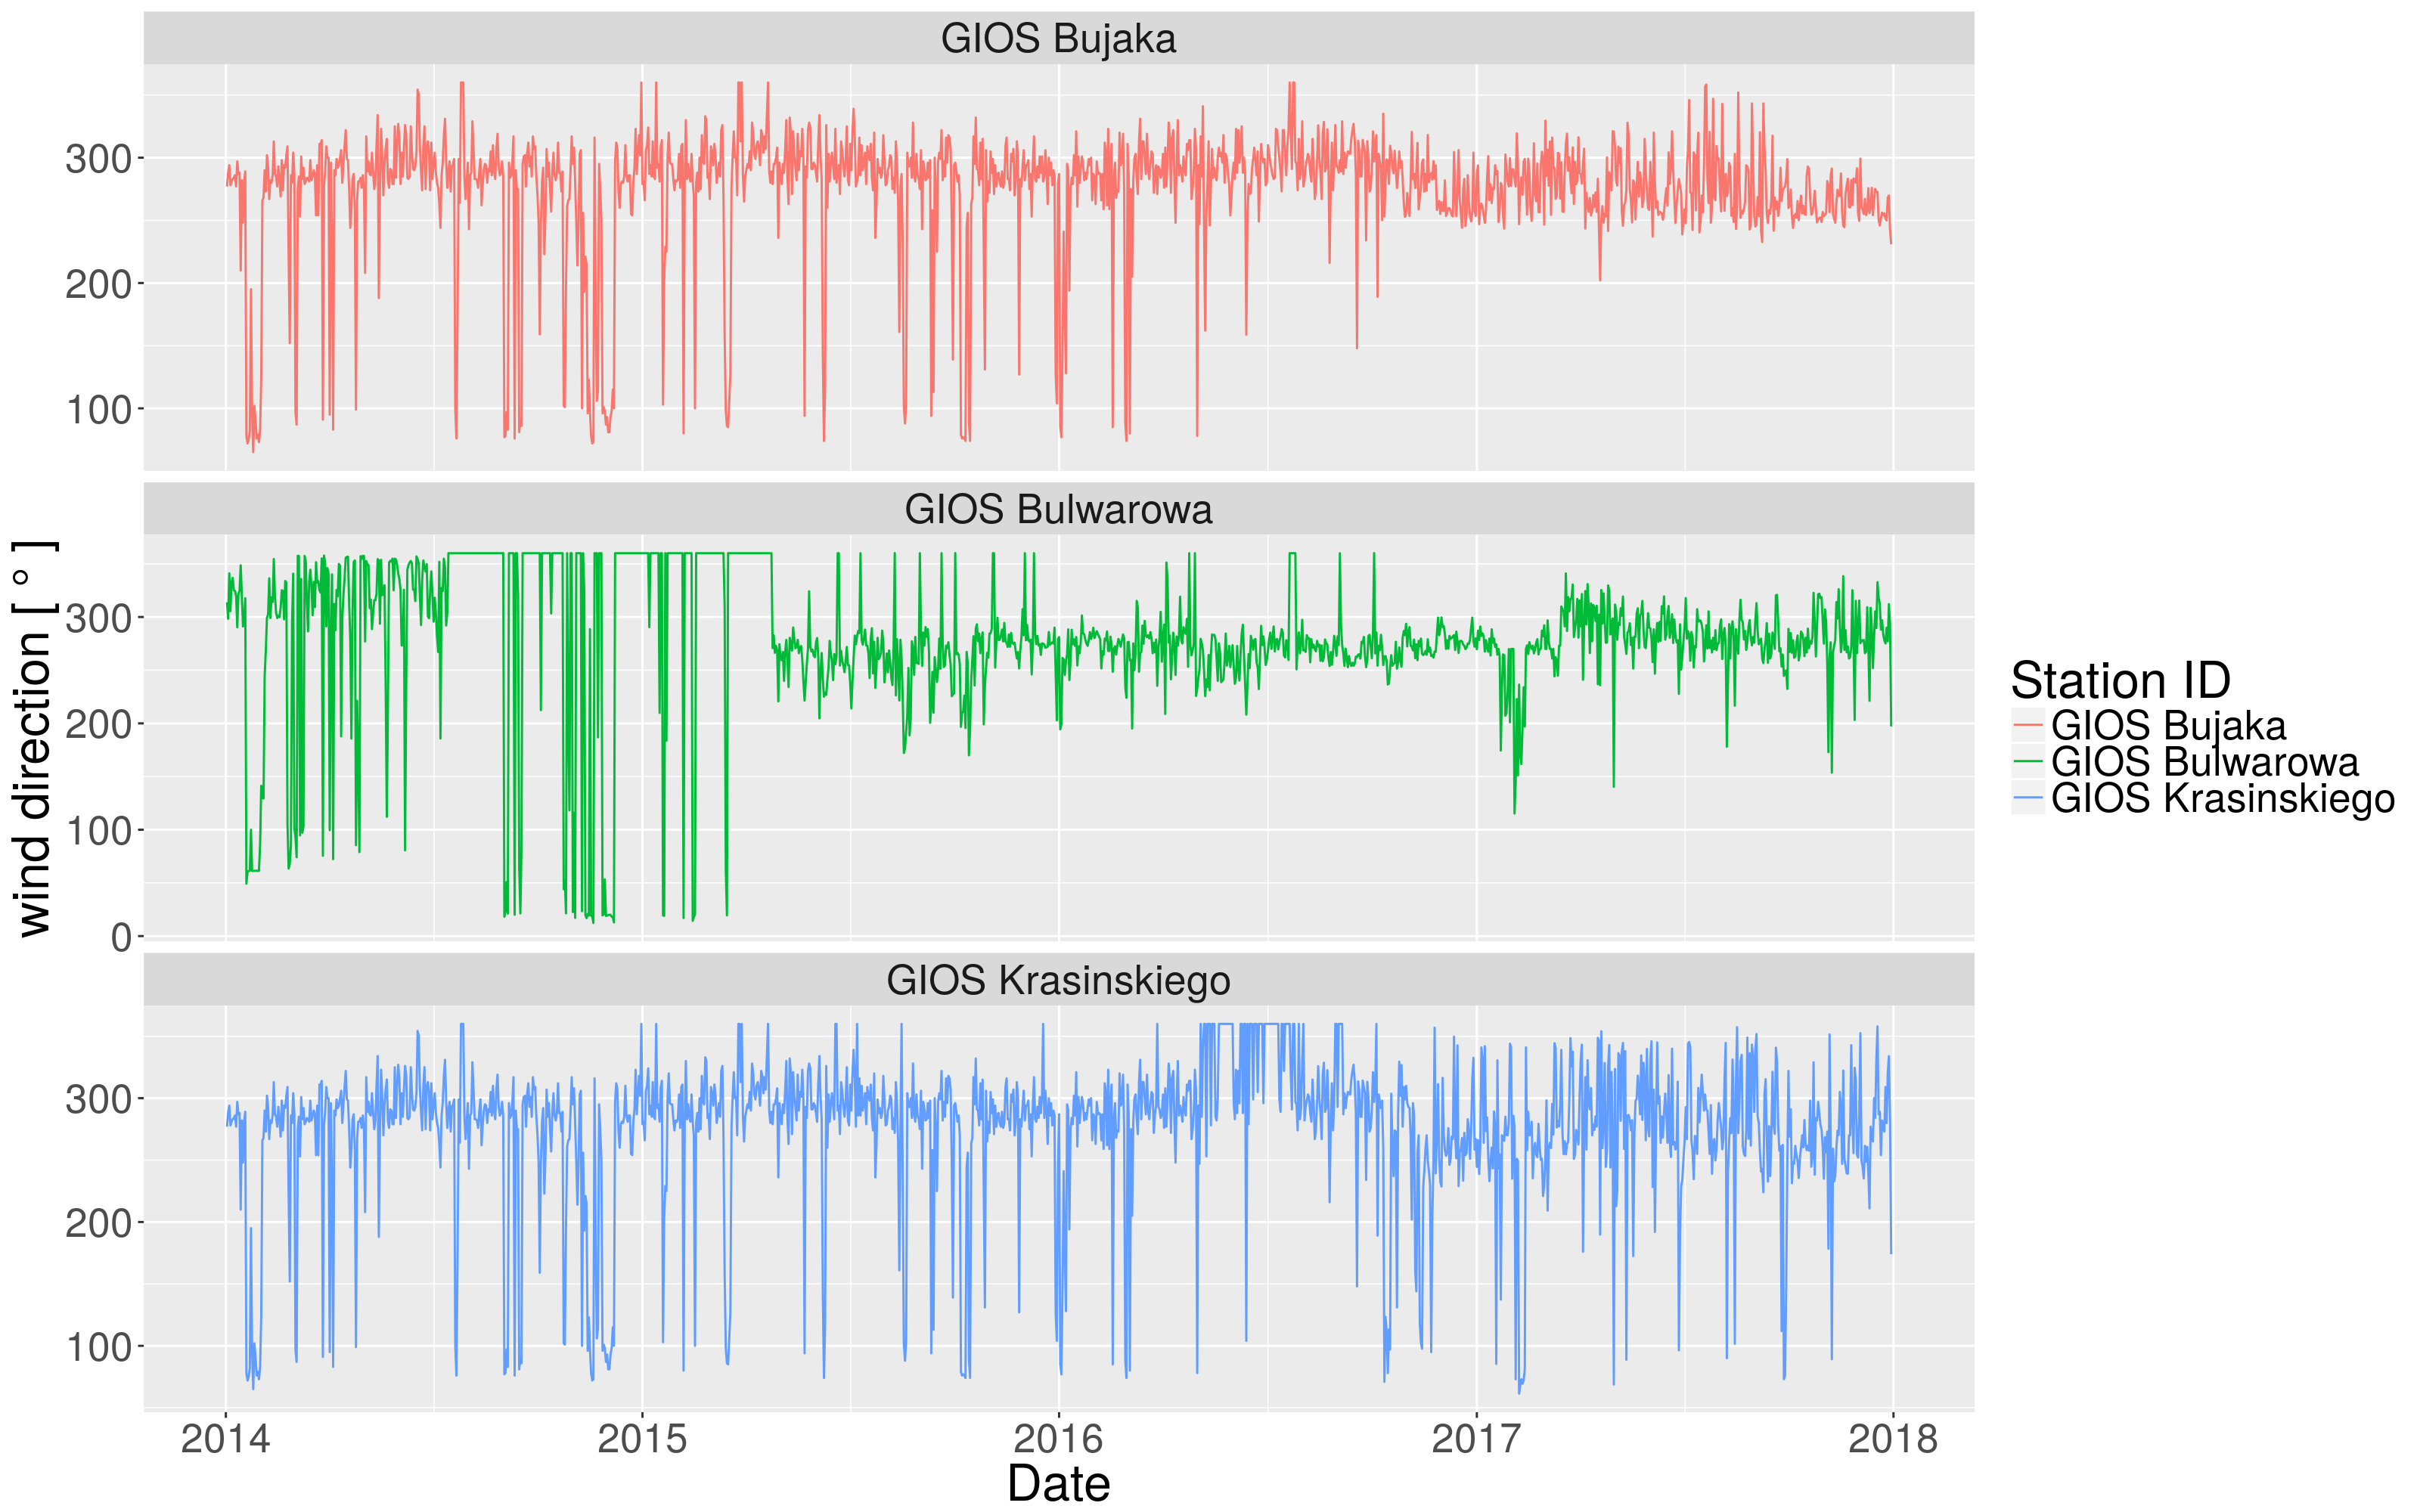
\includegraphics[width=\linewidth]{figures/dataset/trend/wind_dir_deg_yearly_trend.png}
  \caption{Mean daily wind direction}
  \label{fig:dataset-trend-wind-dir-ew}
  \end{figure}
\end{landscape}
\begin{landscape}
\begin{figure}[htp]
\centering
  \centering
  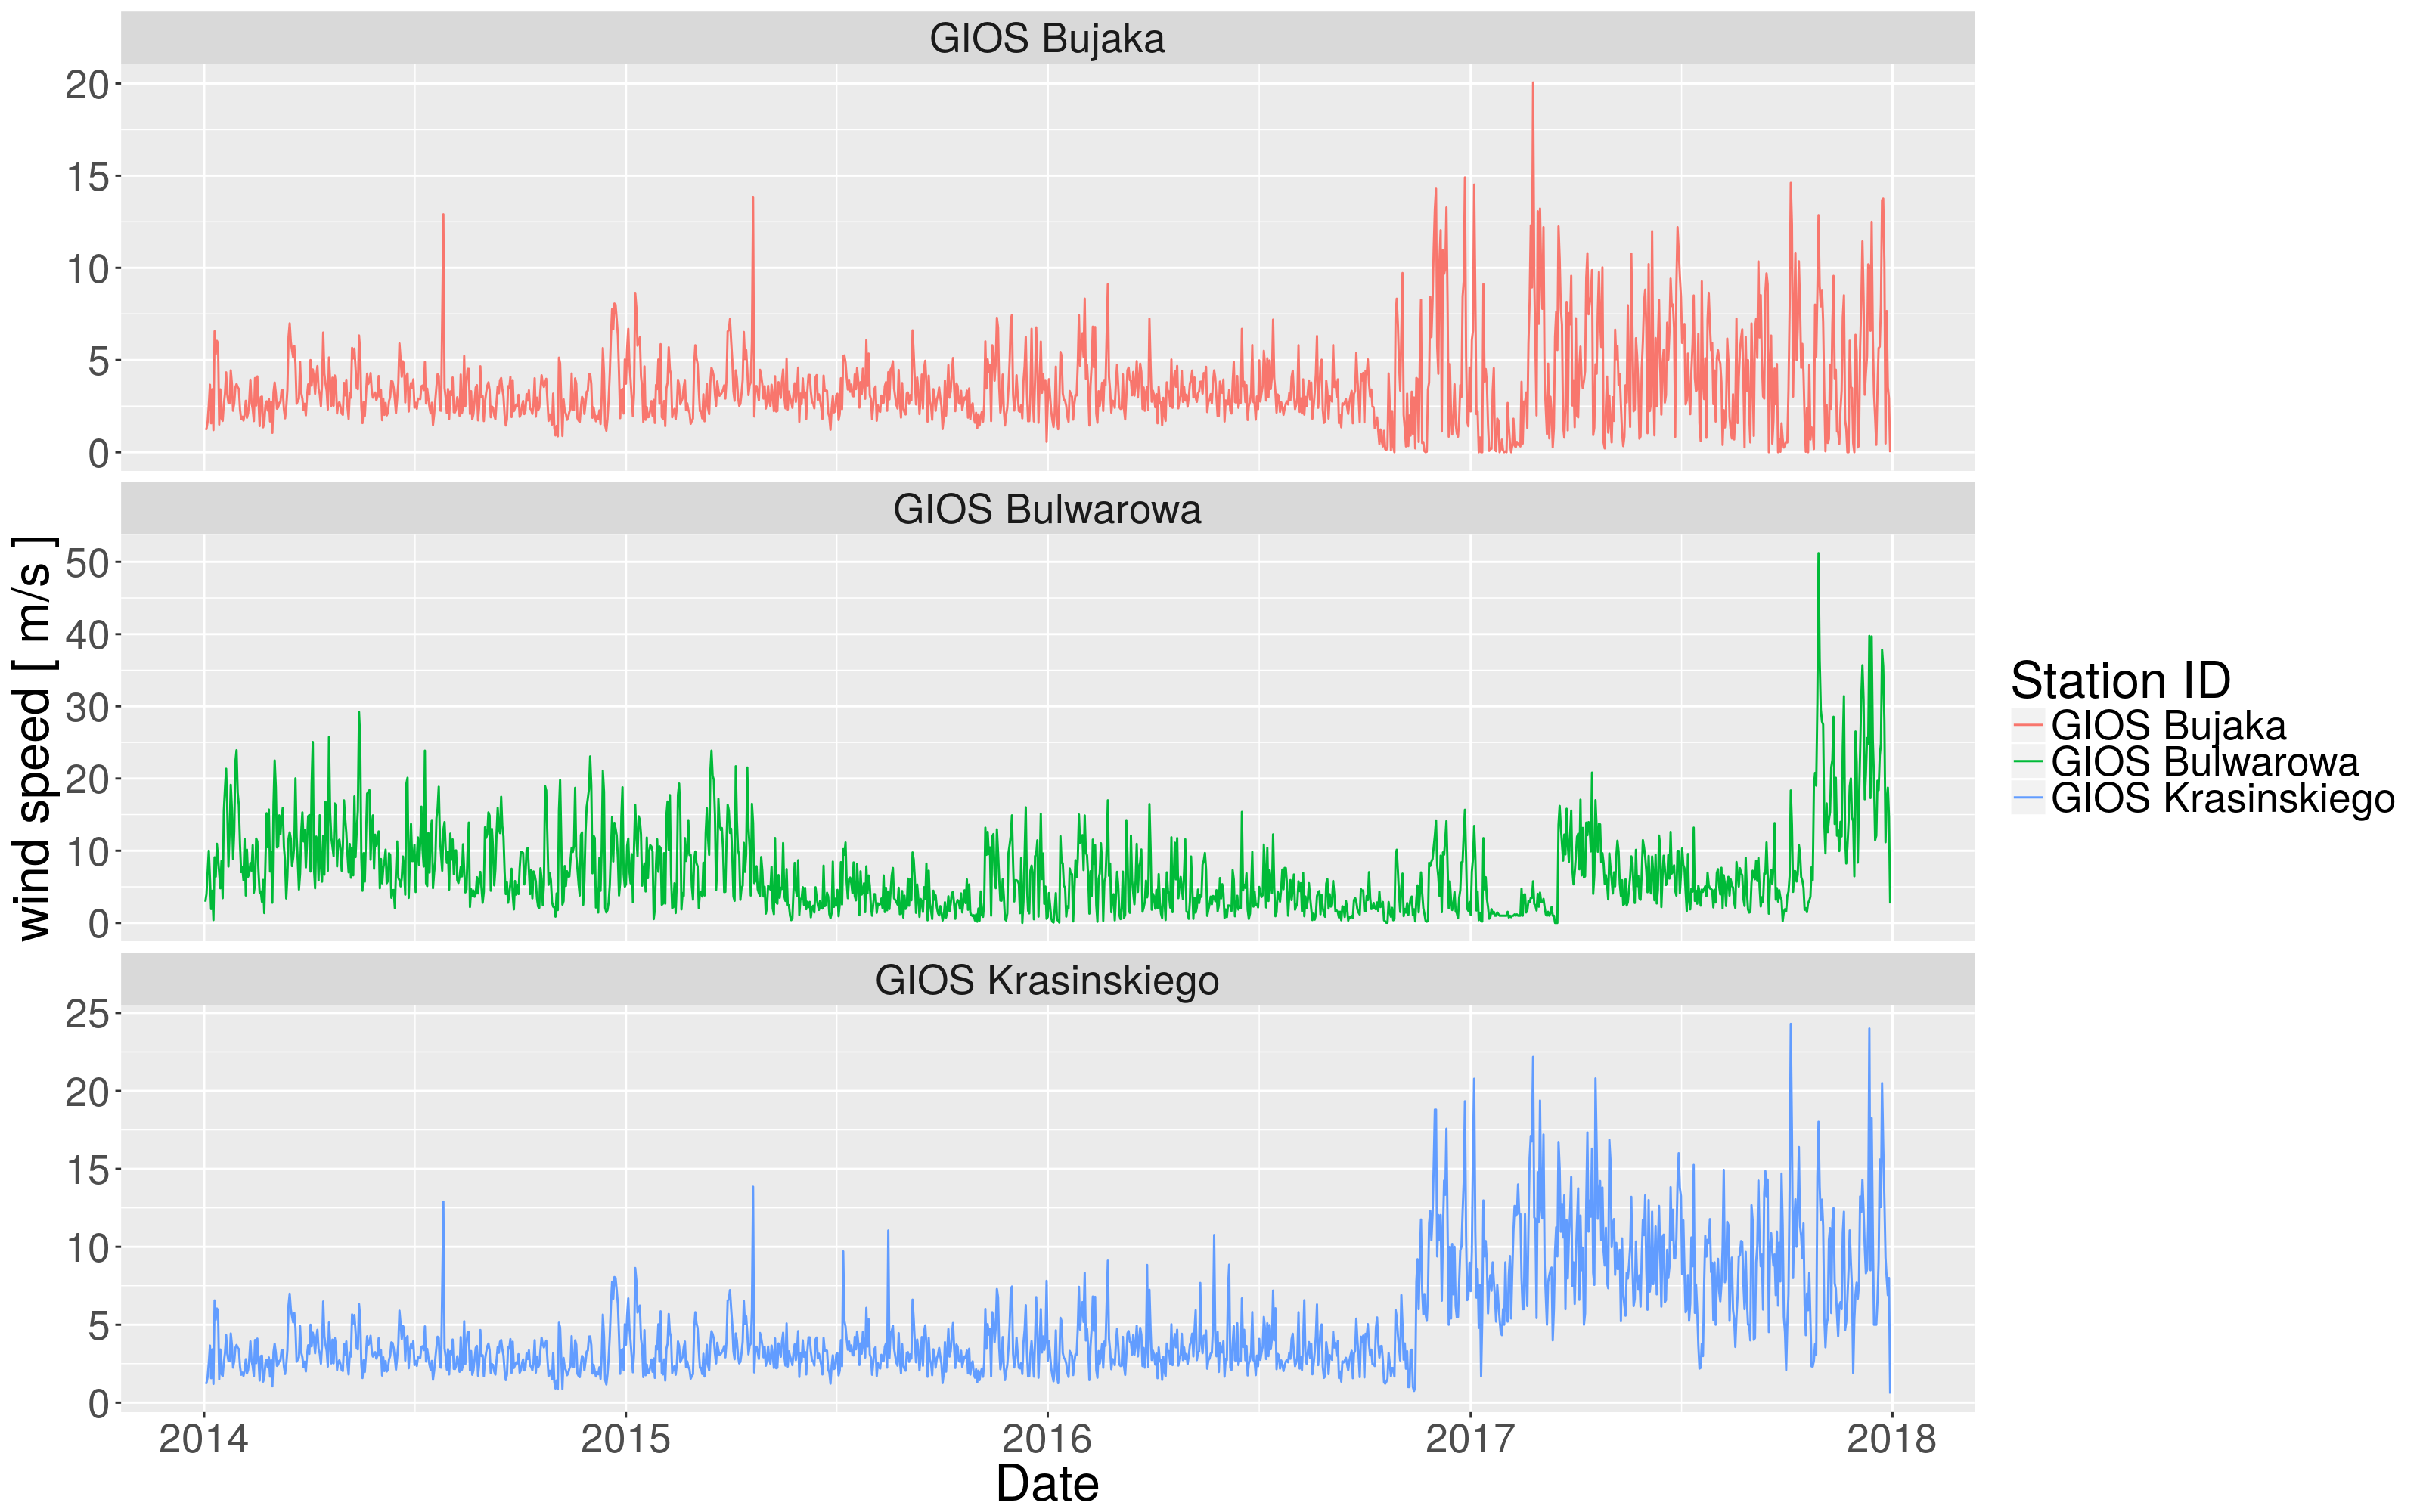
\includegraphics[width=\linewidth]{figures/dataset/trend/wind_speed_yearly_trend.png}
  \caption{Mean daily wind speed}
  \label{fig:dataset-trend-wind-speed}
  \end{figure}
\end{landscape}

% BI-VARIATE SCATTER PLOTS %

\begin{landscape}
\begin{figure}[htp]
\centering
  \centering
  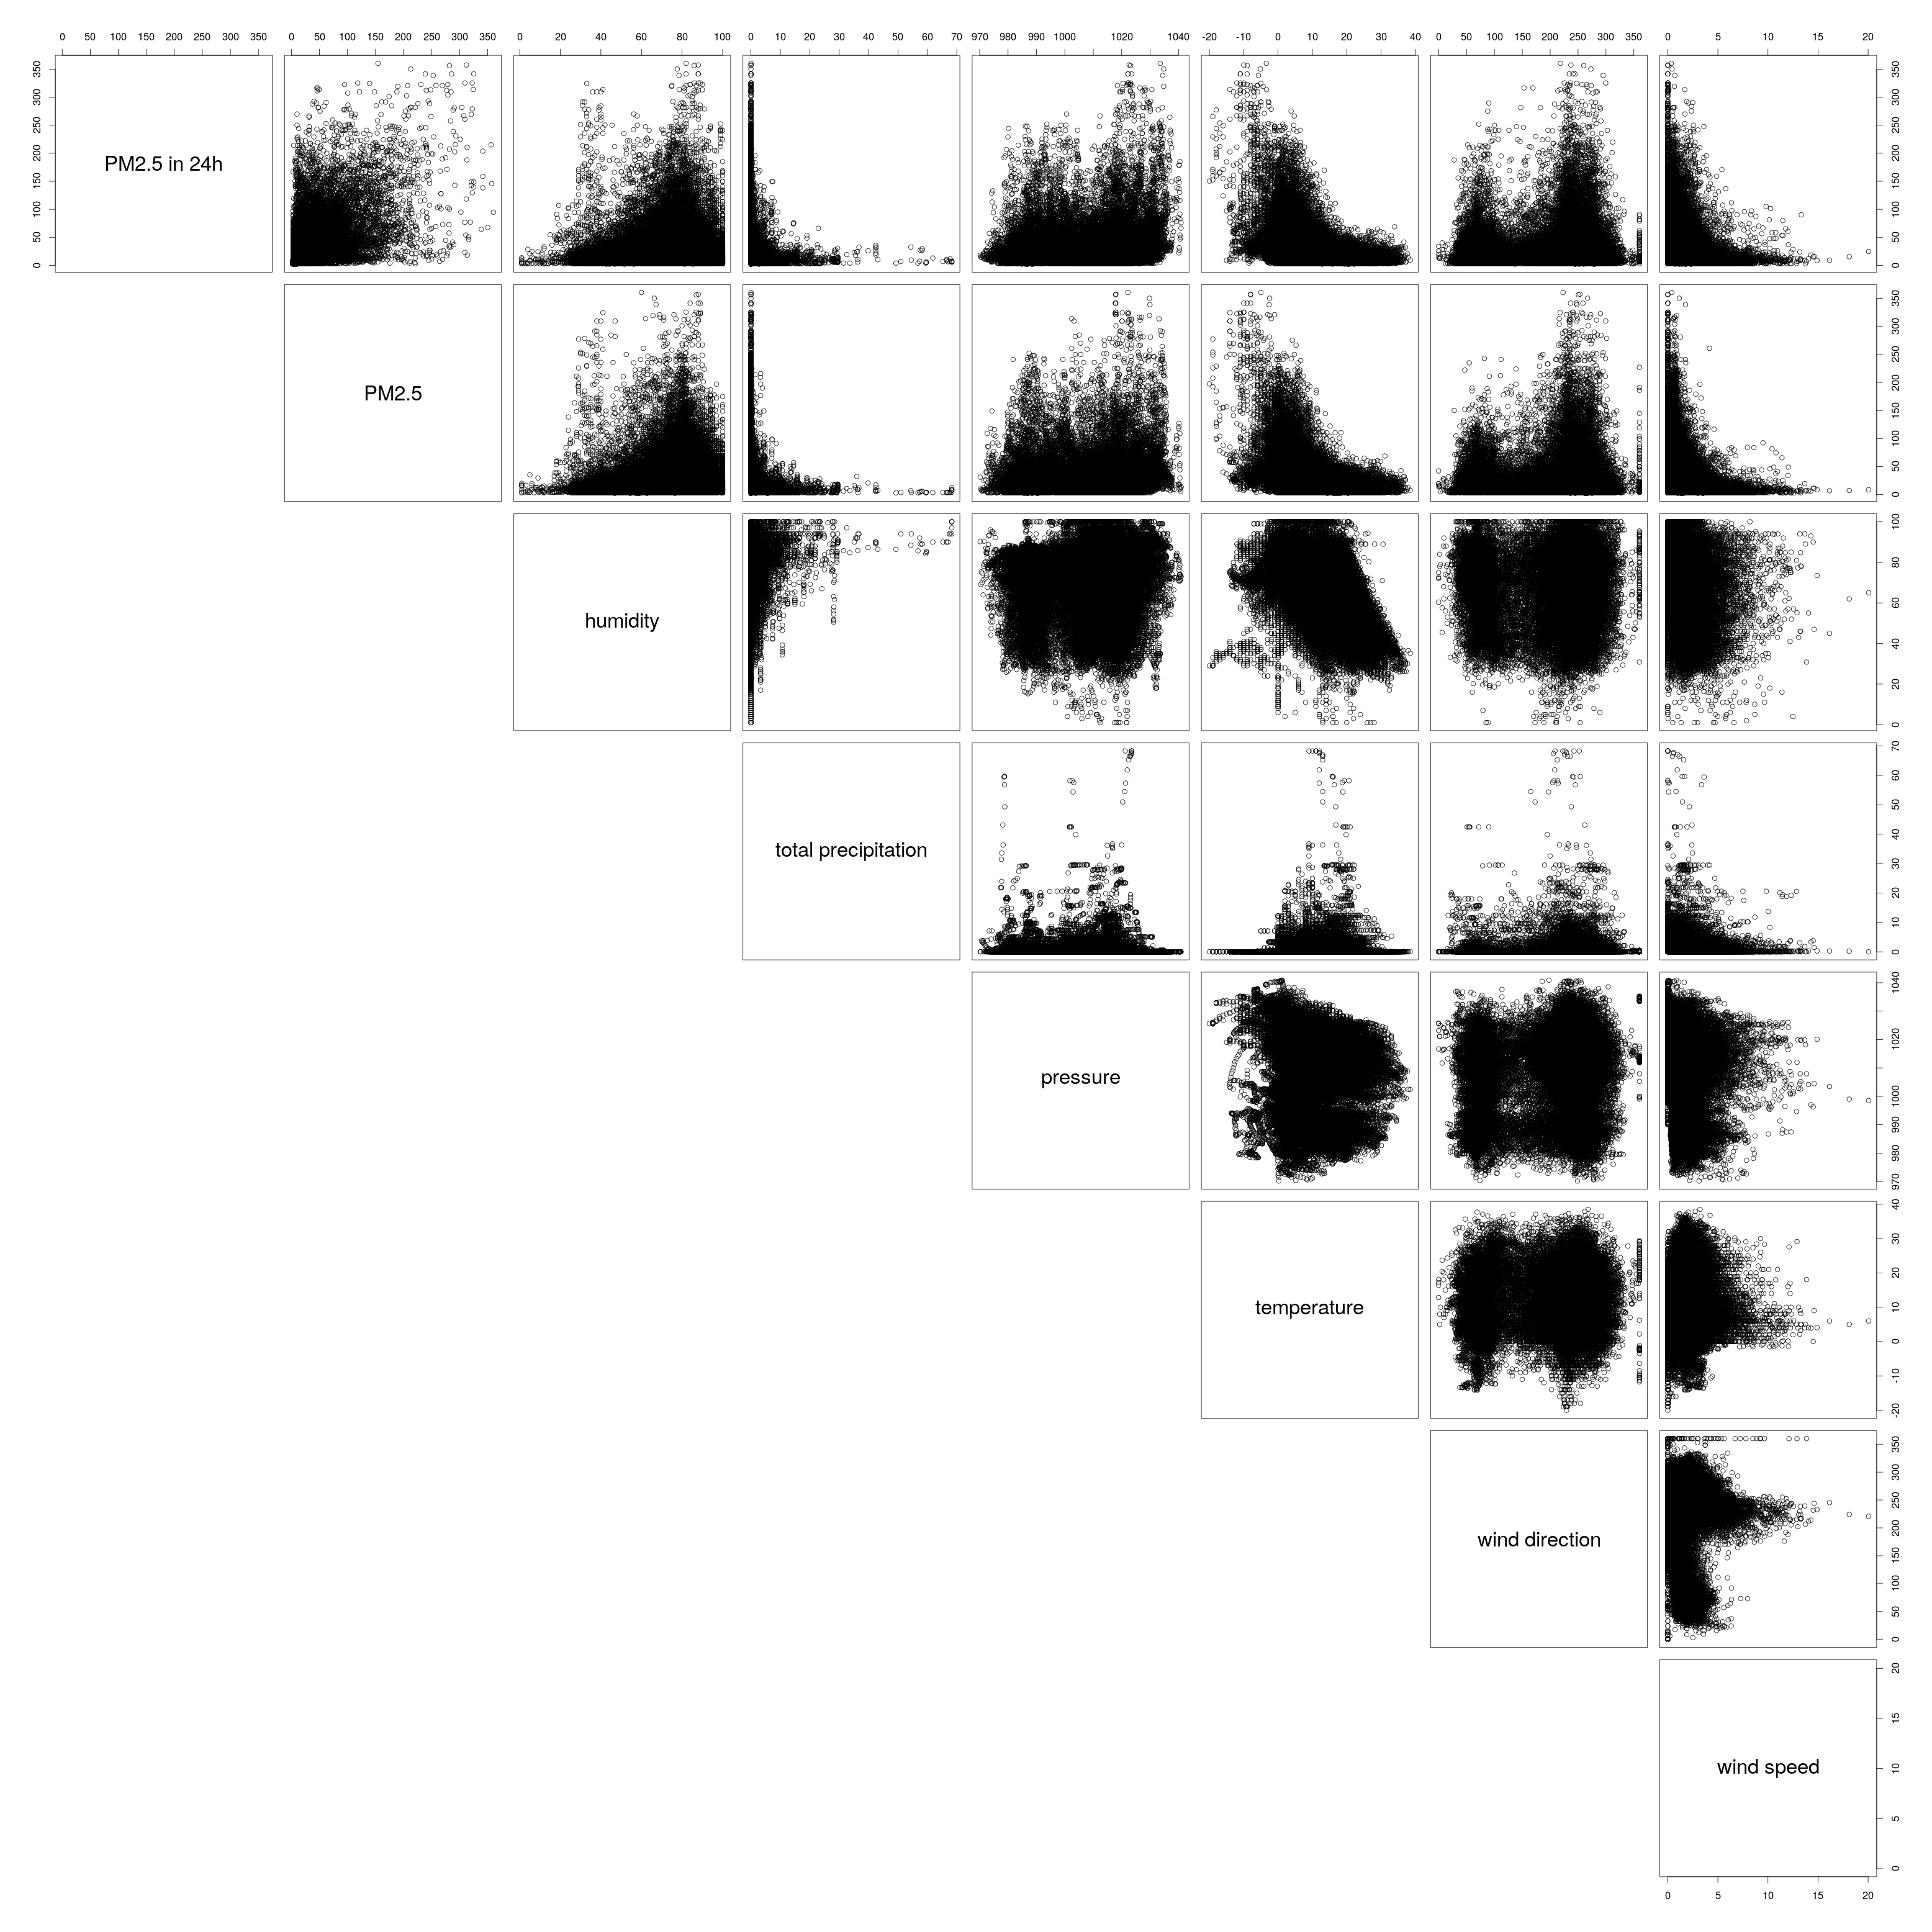
\includegraphics[width=0.65\linewidth]{figures/dataset/bivariate/relationships_gios_bujaka.png}
  \caption{Bivariate relationships - GIOŚ Bujaka}
  \label{fig:dataset-bivariate-bujaka}
\end{figure}
\end{landscape}
\begin{landscape}
\begin{figure}[htp]
\centering
  \centering
    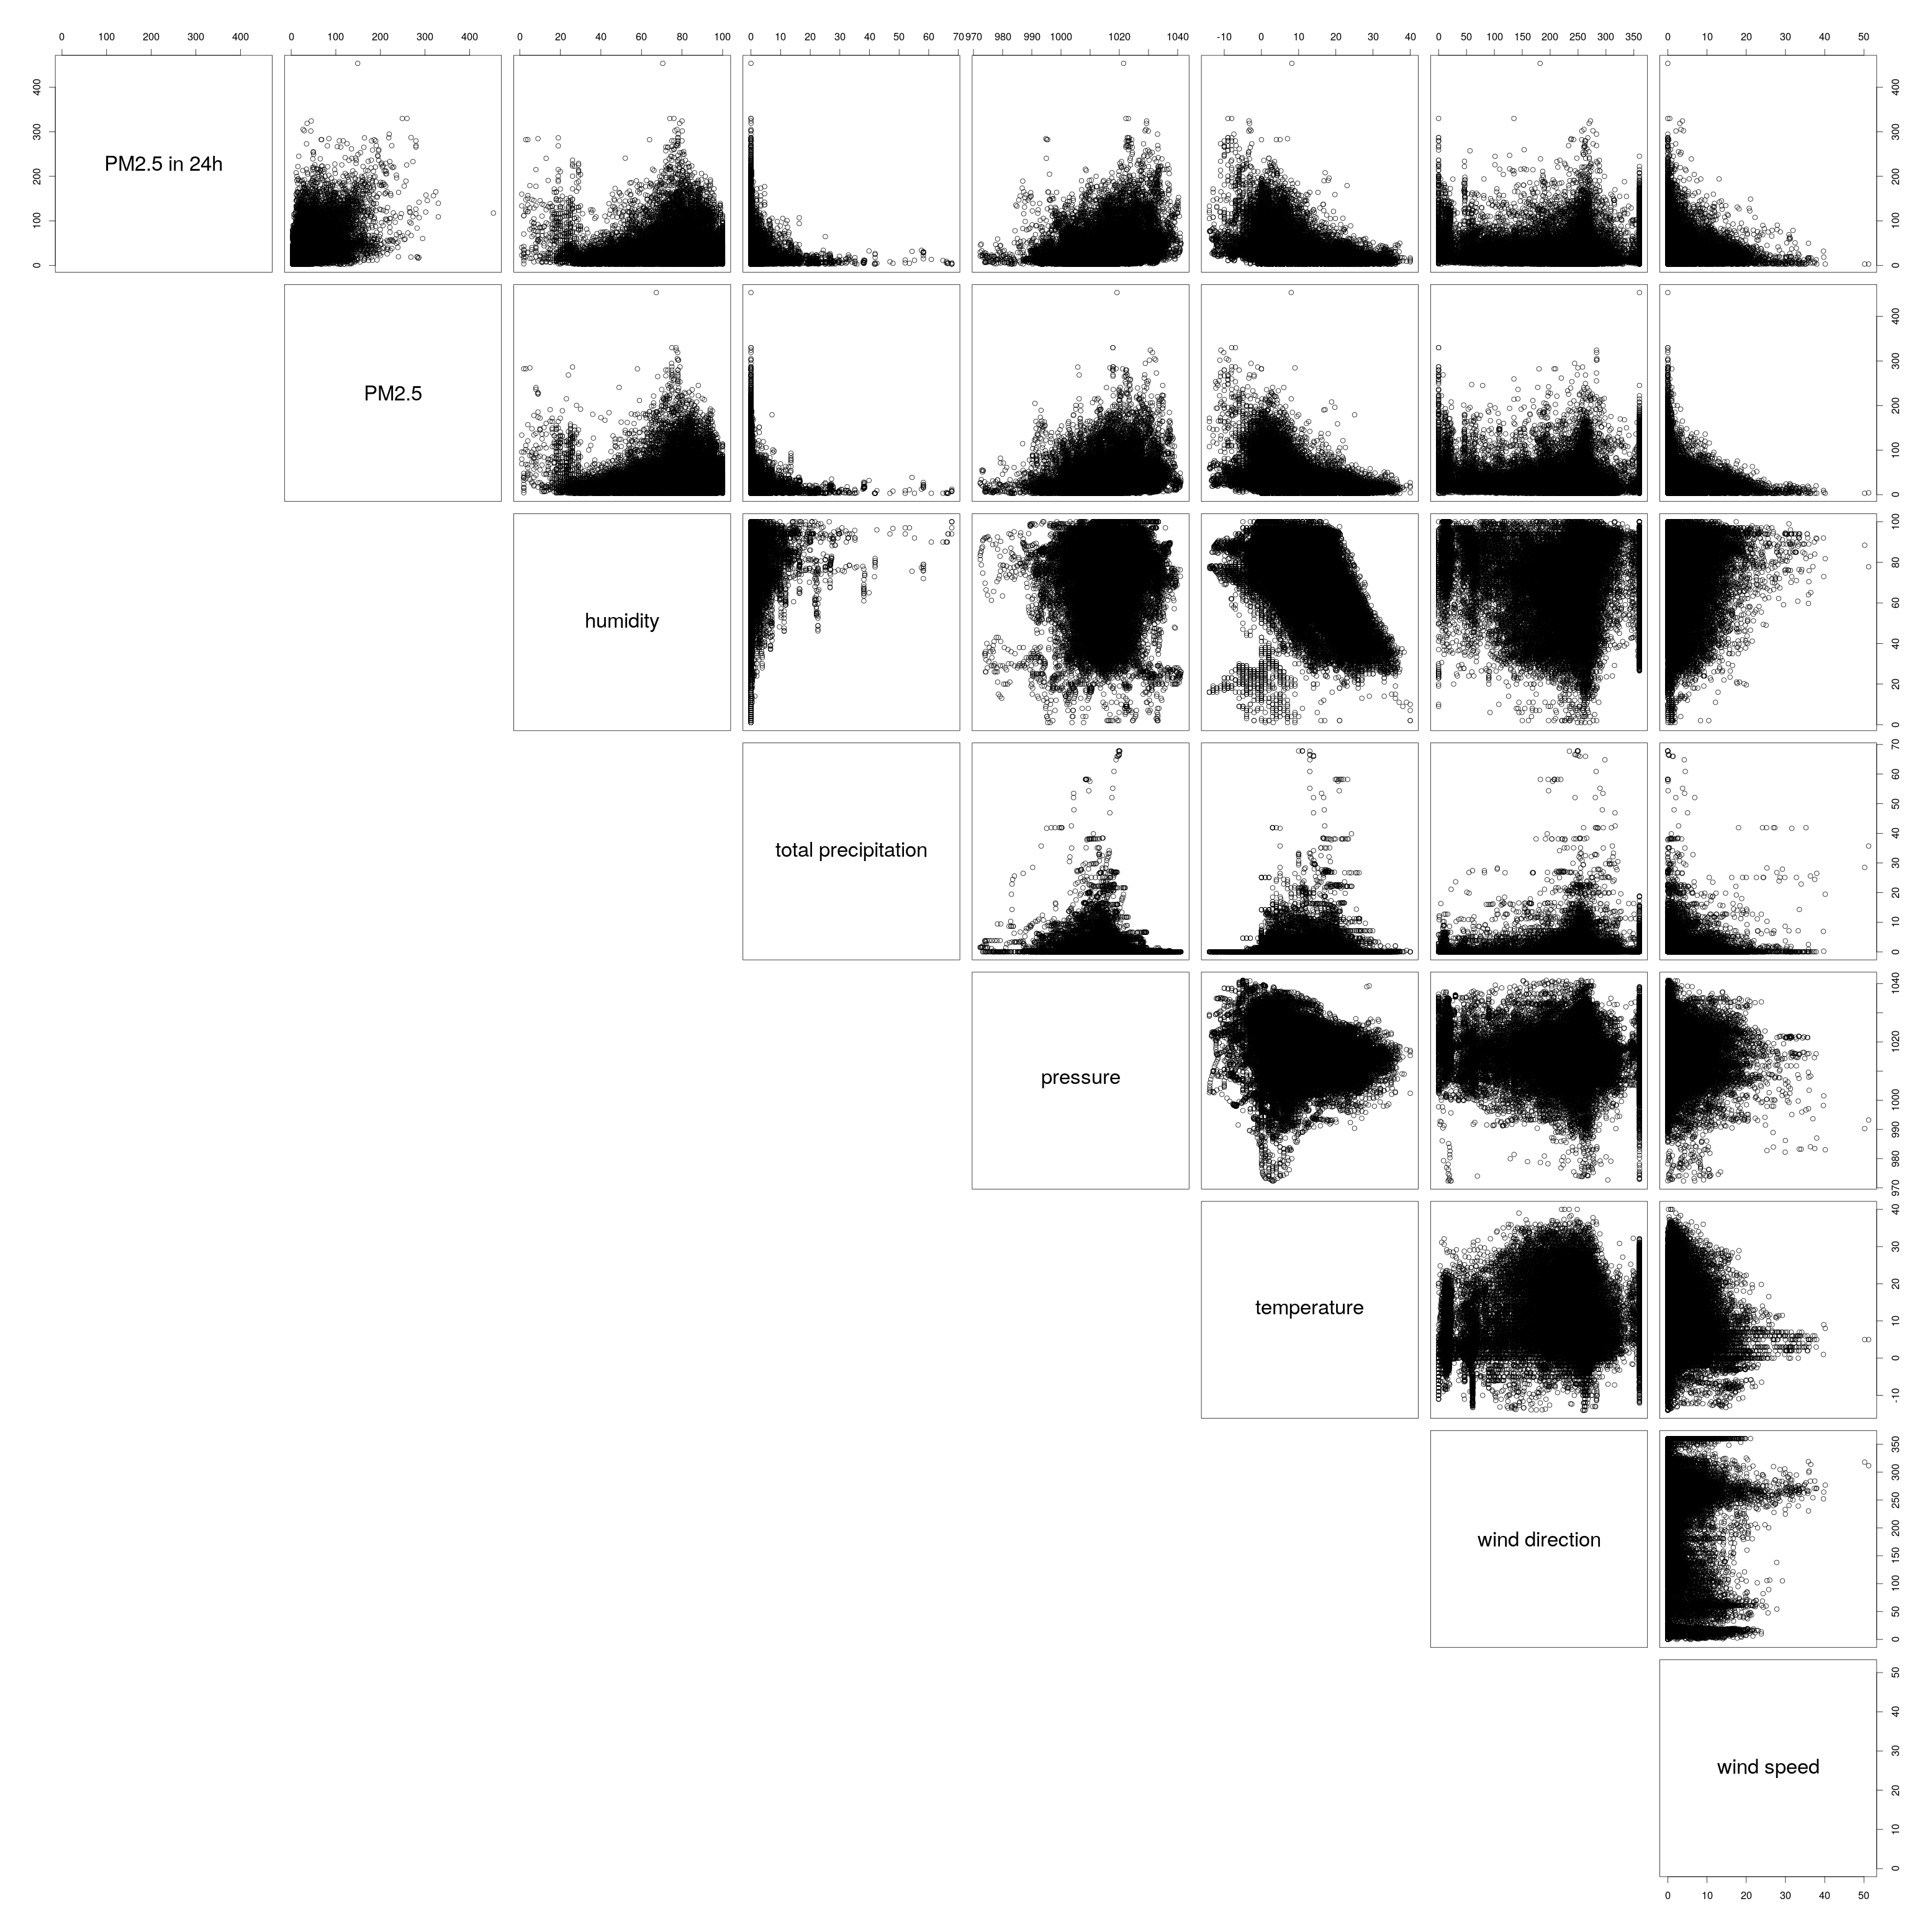
\includegraphics[width=0.65\linewidth]{figures/dataset/bivariate/relationships_gios_bulwarowa.png}
    \caption{Bivariate relationships - GIOŚ Bulwarowa}
    \label{fig:dataset-bivariate-bulwarowa}
\end{figure}
\end{landscape}
\begin{landscape}
\begin{figure}[htp]
\centering
  \centering
  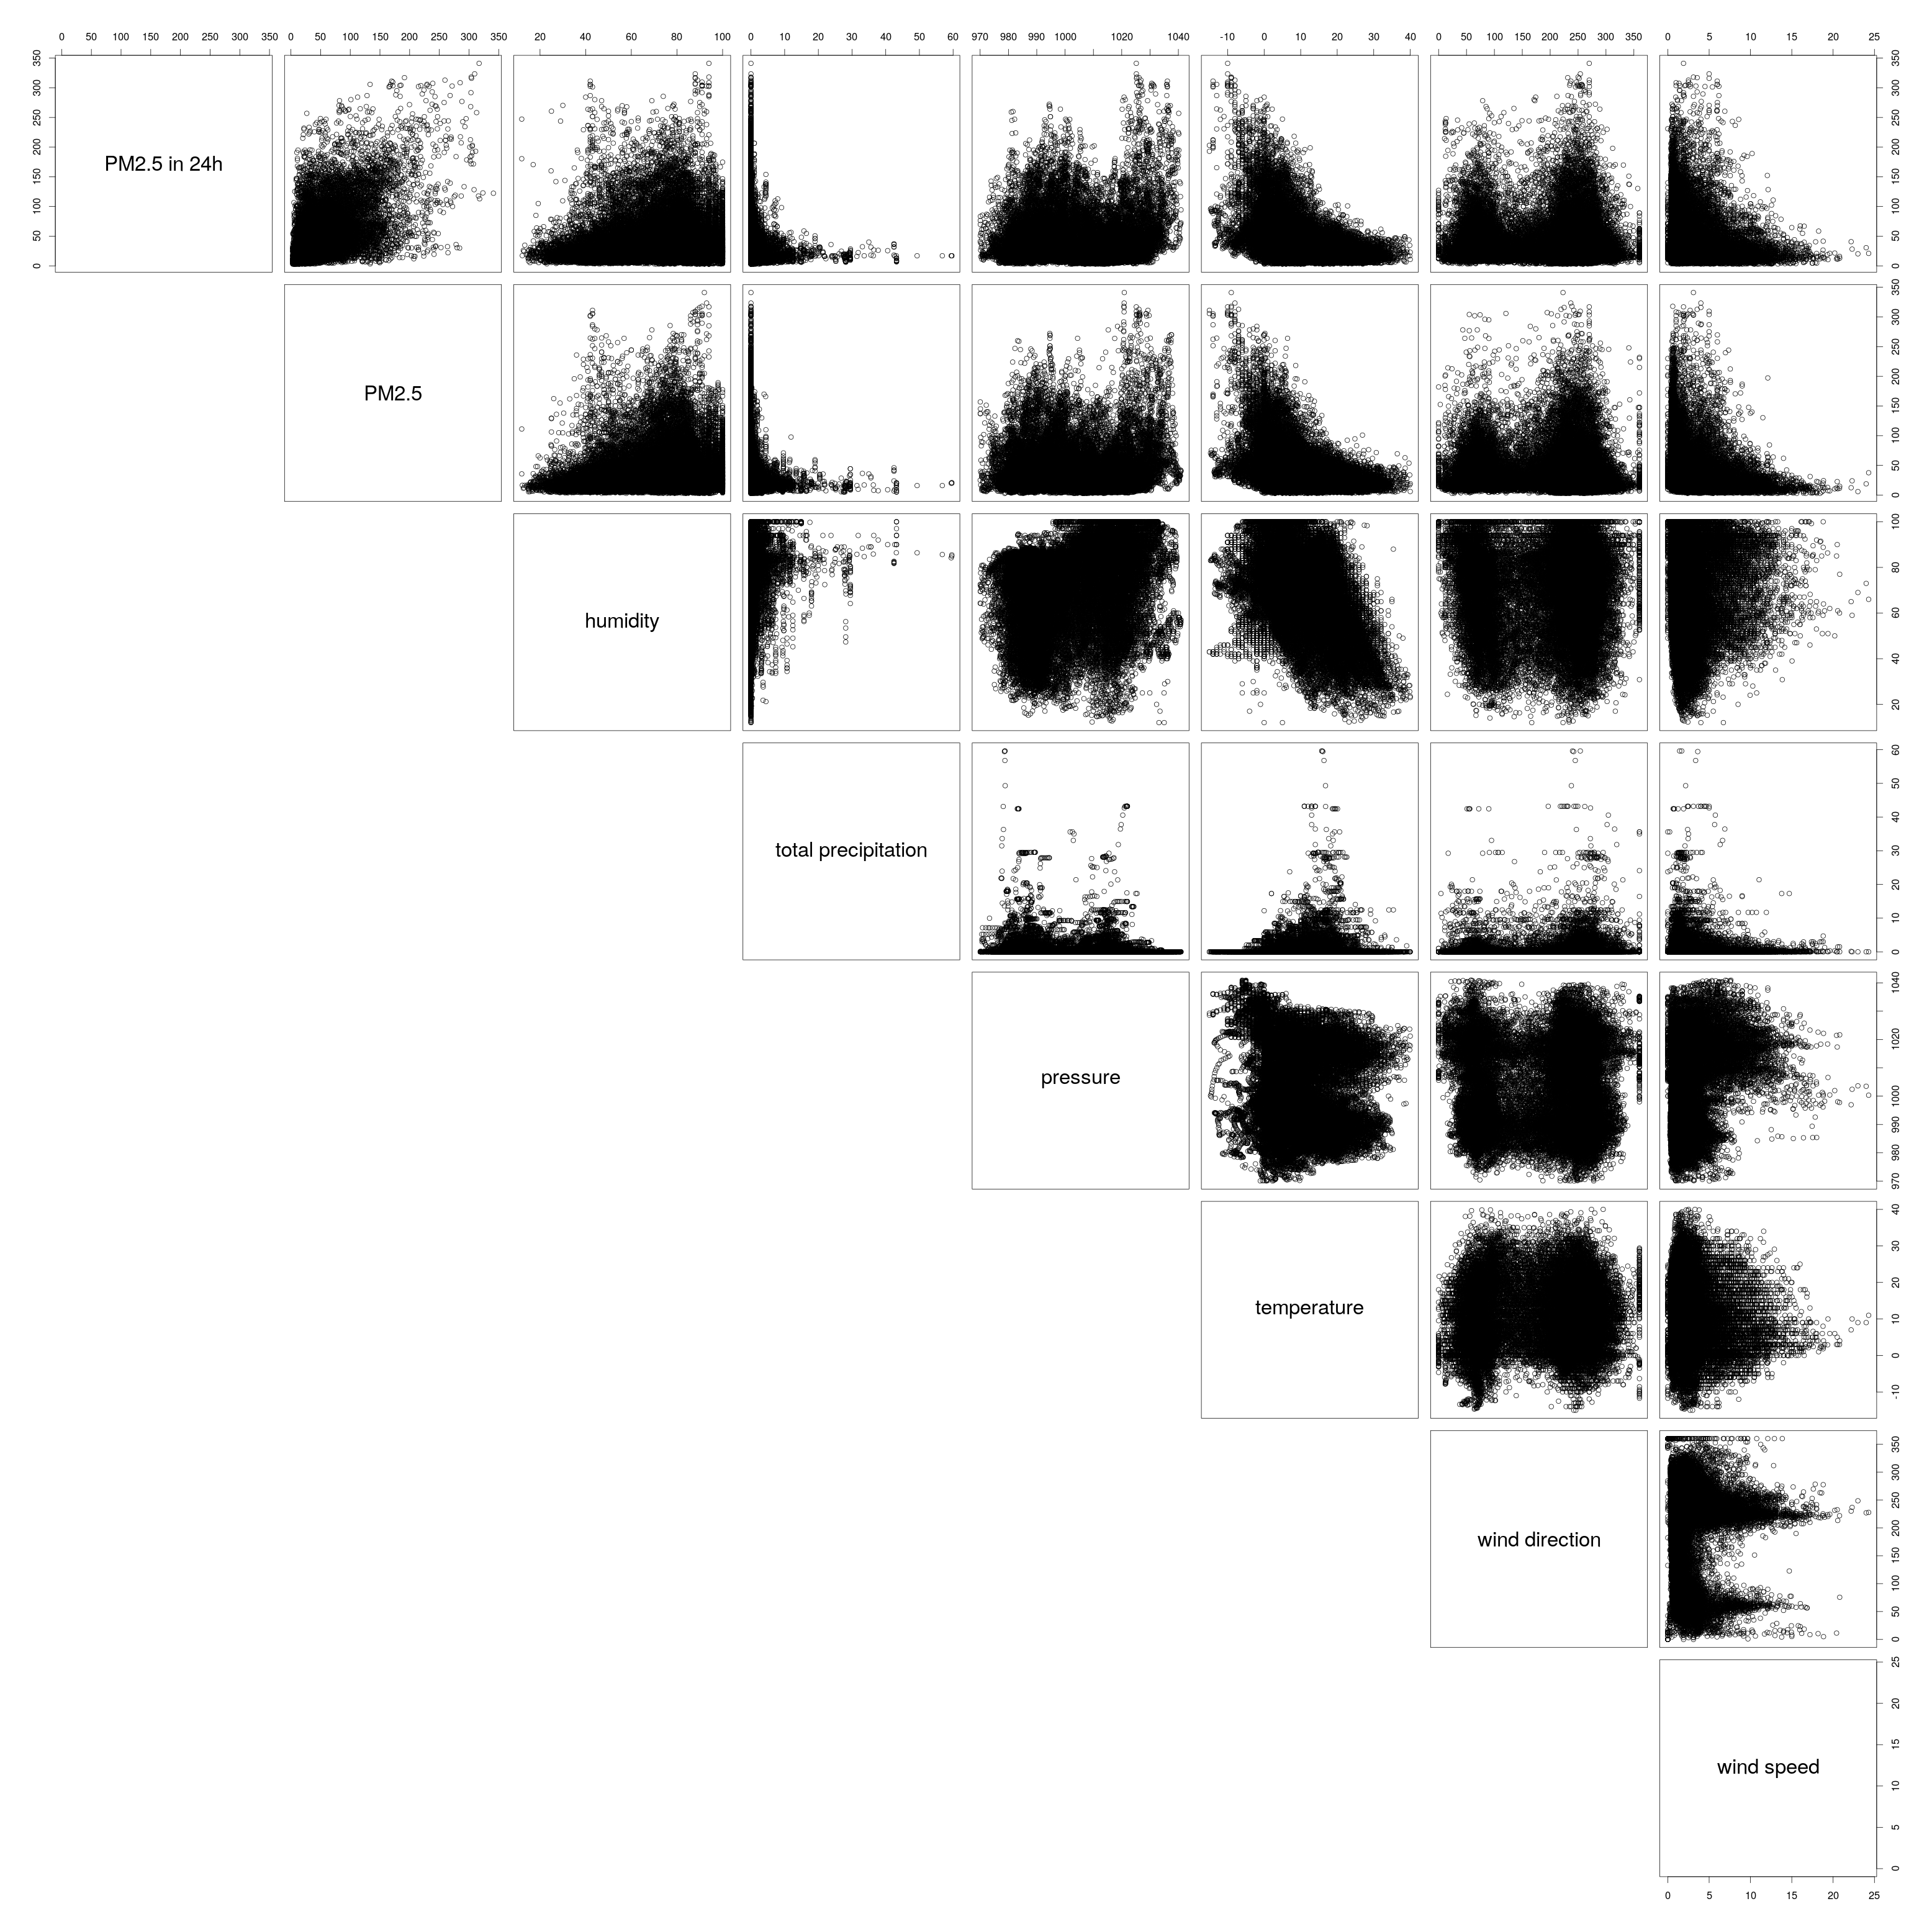
\includegraphics[width=0.65\linewidth]{figures/dataset/bivariate/relationships_gios_krasinskiego.png}
  \caption{Bivariate relationships - GIOŚ Krasińskiego}
  \label{fig:dataset-bivariate-krasinskiego}
  \end{figure}
\end{landscape}

% CORRELATION %

% \begin{figure}[htp]
% \centering
%       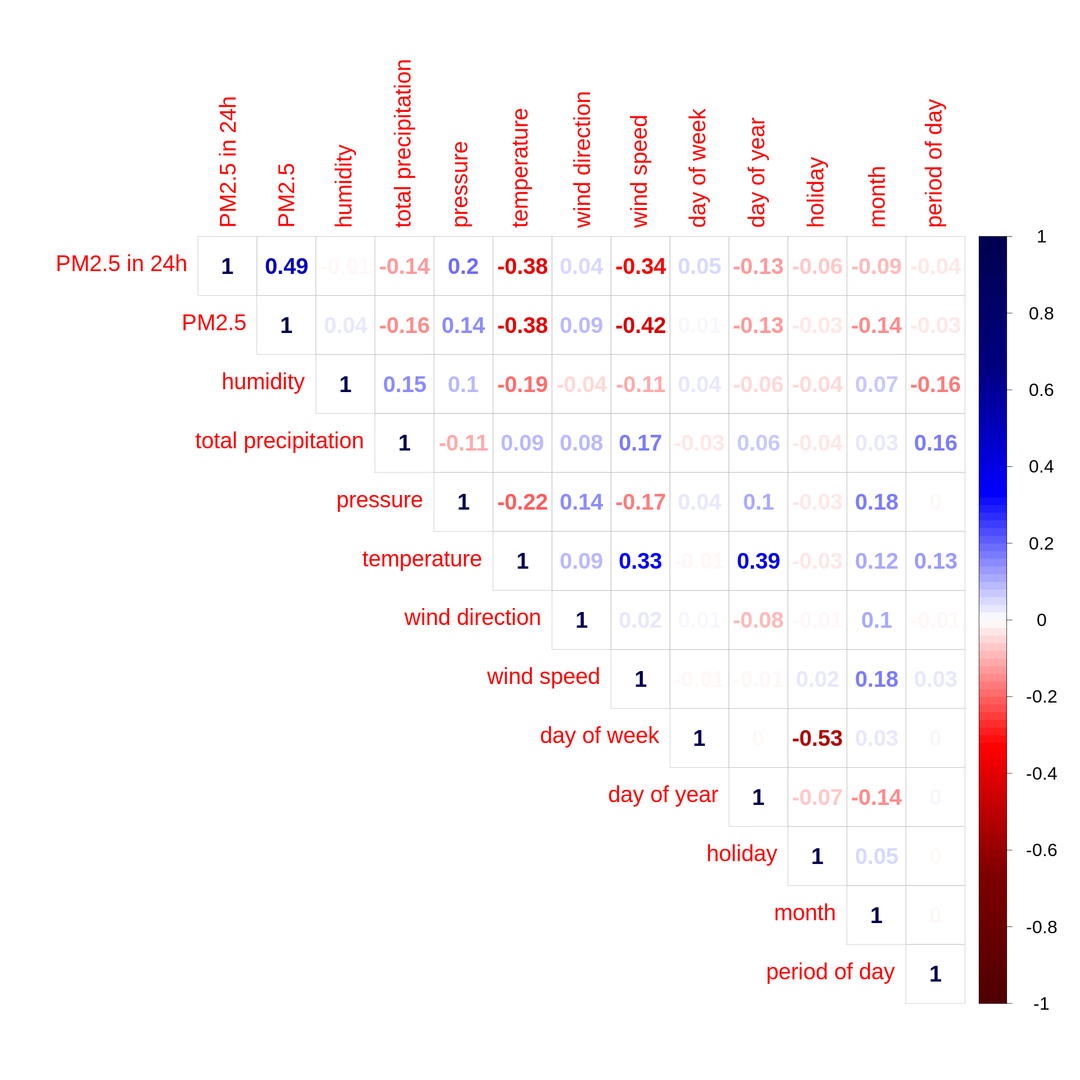
\includegraphics[width=\linewidth]{figures/dataset/correlation/corrplot_gios_bujaka_1.png}
%       \caption{Correlation plots - winter, GIOŚ Bujaka}
%       \label{fig:dataset-correlation-winter-bujaka}
% \end{figure}
% \begin{figure}[htp]
% \centering
%       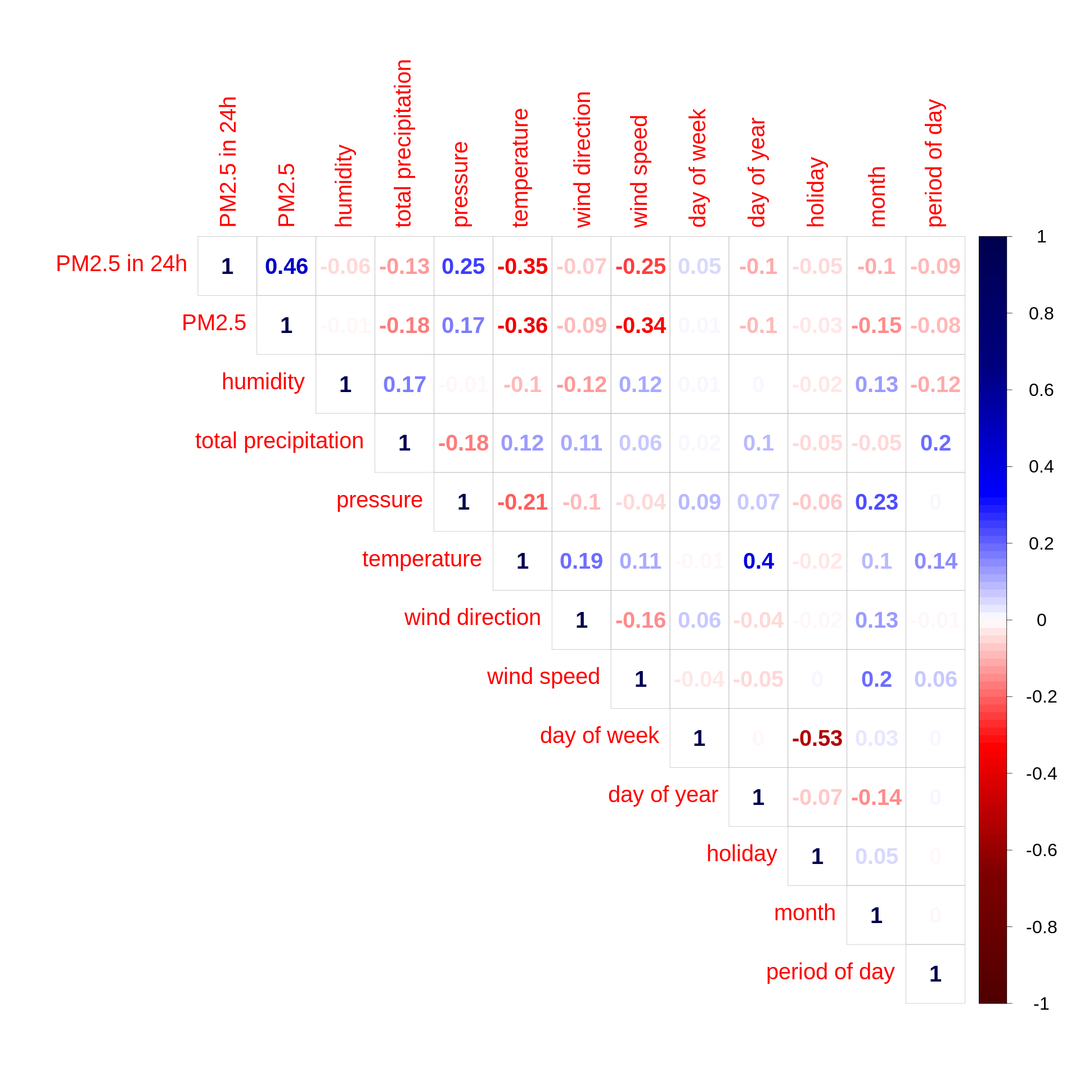
\includegraphics[width=\linewidth]{figures/dataset/correlation/corrplot_gios_bulwarowa_1.png}
%       \caption{Correlation plots - winter, GIOŚ Bulwarowa}
%       \label{fig:dataset-correlation-winter-bulwarowa}
% \end{figure}
% \begin{figure}[htp]
% \centering
%       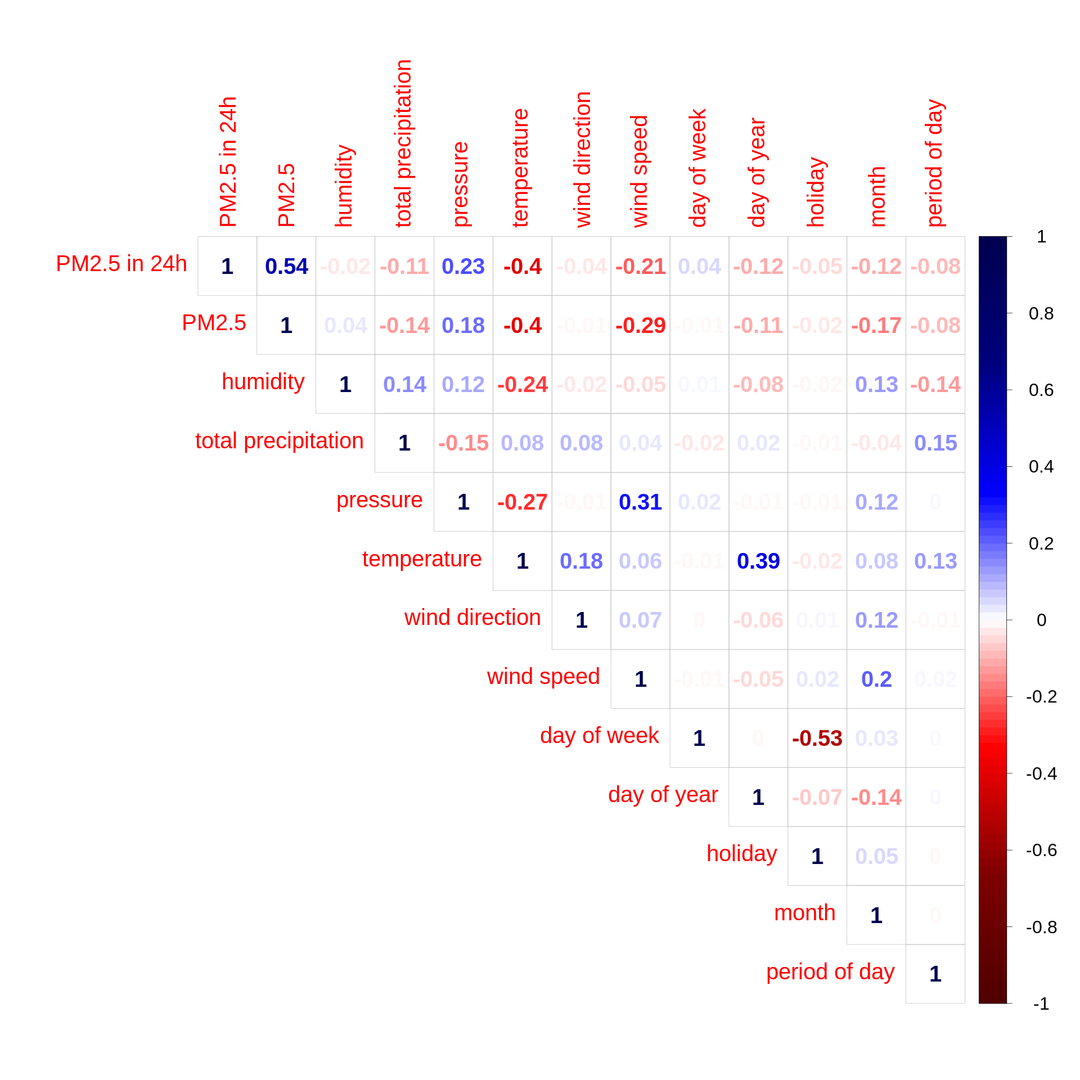
\includegraphics[width=\linewidth]{figures/dataset/correlation/corrplot_gios_krasinskiego_1.png}
%       \caption{Correlation plots - winter, GIOŚ Krasińskiego}
%       \label{fig:dataset-correlation-winter-krasinskiego}
% \end{figure}

% \begin{figure}[htp]
% \centering
%       \centering
%       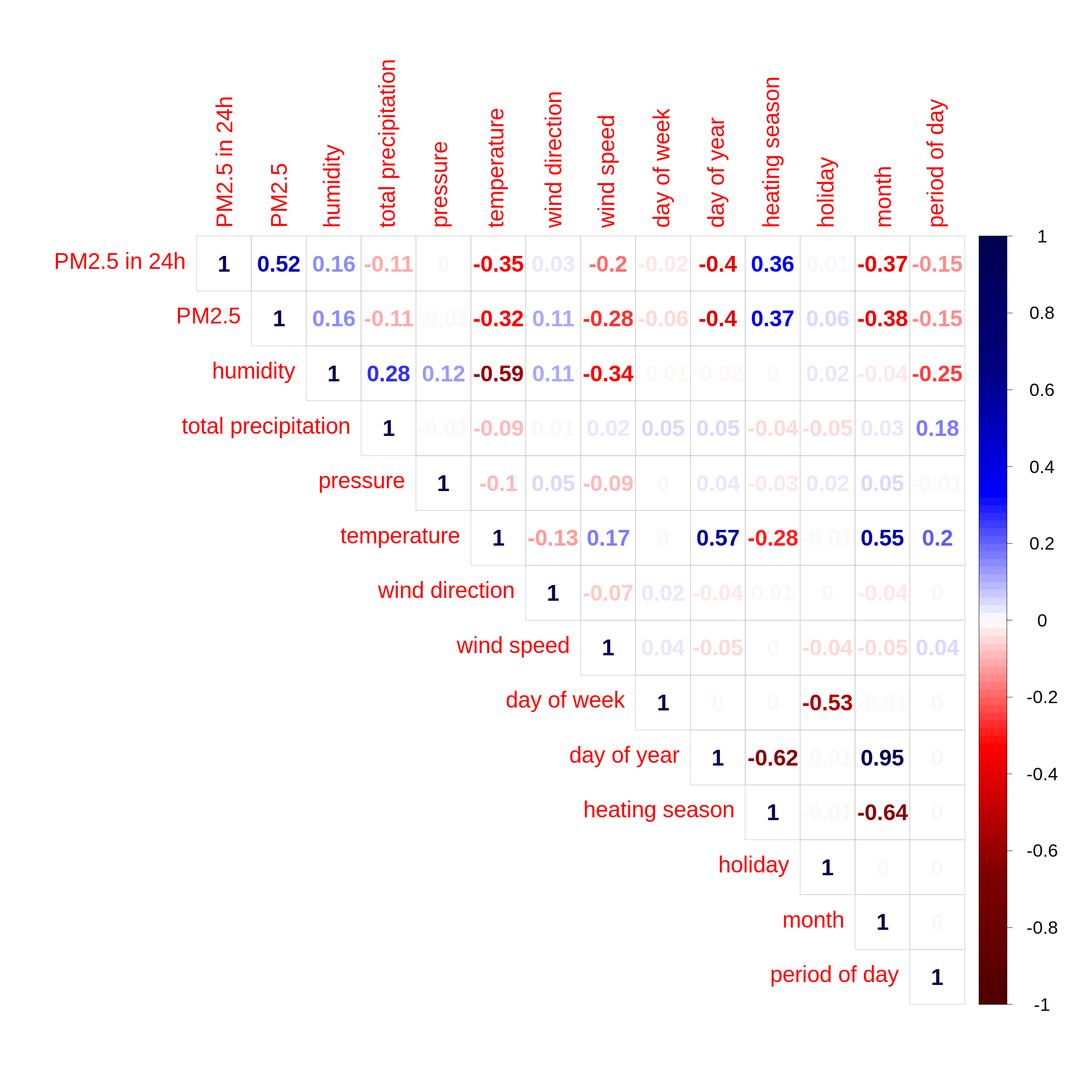
\includegraphics[width=\linewidth]{figures/dataset/correlation/corrplot_gios_bujaka_2.png}
%       \caption{Correlation plots - spring, GIOŚ Bujaka}
%       \label{fig:dataset-correlation-spring-bujaka}
% \end{figure}
% \begin{figure}[htp]
% \centering
%       \centering
%       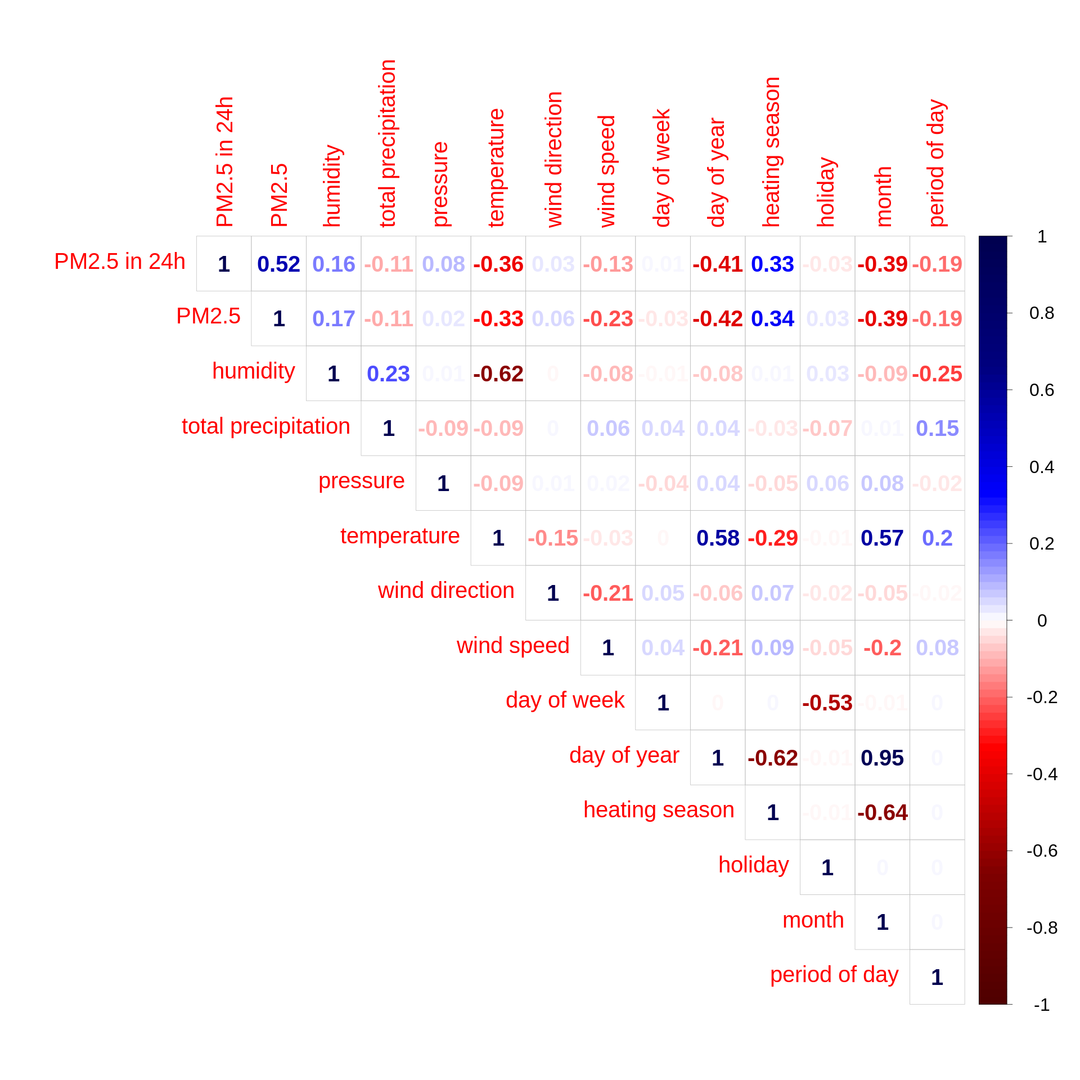
\includegraphics[width=\linewidth]{figures/dataset/correlation/corrplot_gios_bulwarowa_2.png}
%       \caption{Correlation plots - spring, GIOŚ Bulwarowa}
%       \label{fig:dataset-correlation-spring-bulwarowa}
% \end{figure}
% \begin{figure}[htp]
% \centering
%       \centering
%       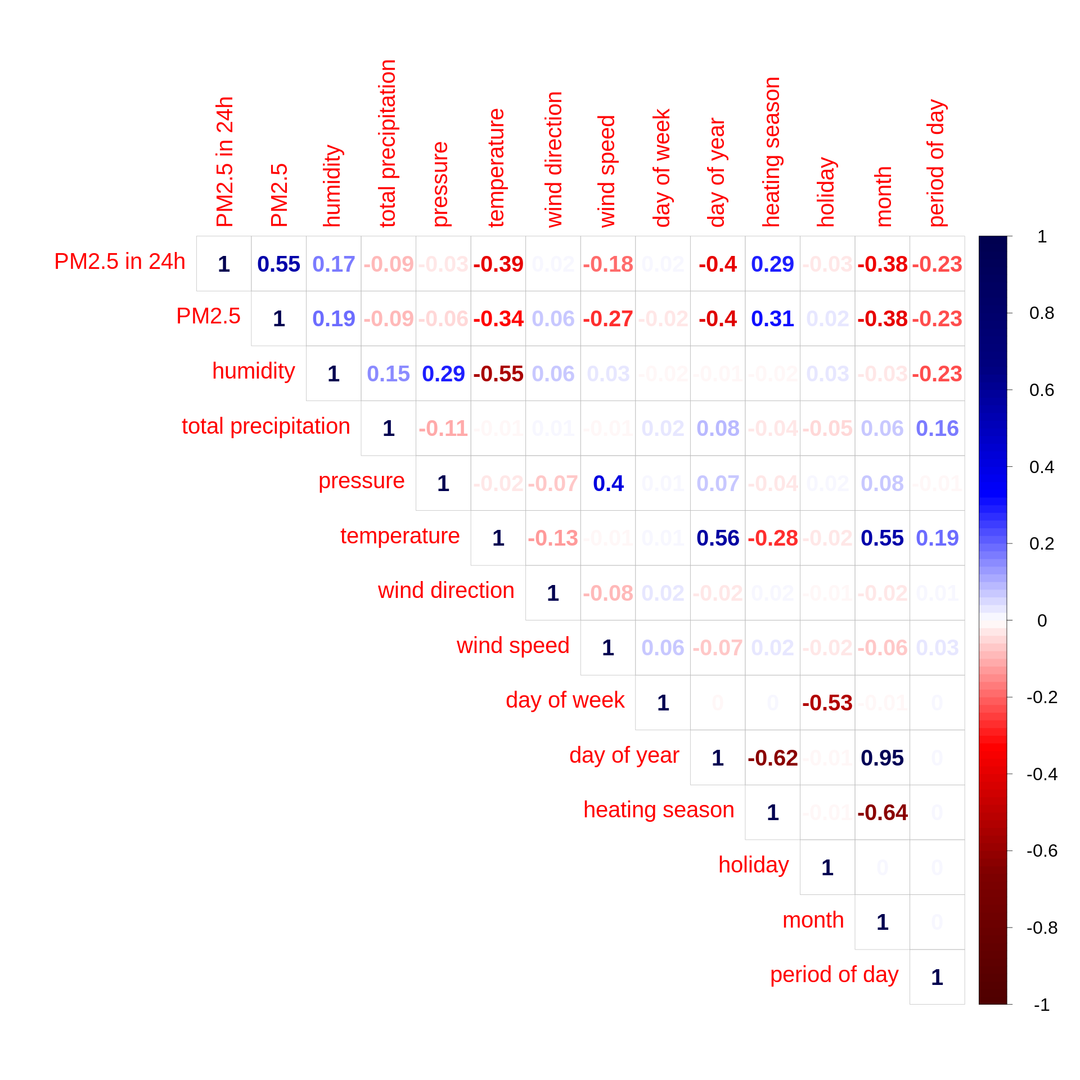
\includegraphics[width=\linewidth]{figures/dataset/correlation/corrplot_gios_krasinskiego_2.png}
%       \caption{Correlation plots - spring, GIOŚ Krasińskiego}
%       \label{fig:dataset-correlation-spring-krasinskiego}
% \end{figure}

% \begin{figure}[htp]
% \centering
%       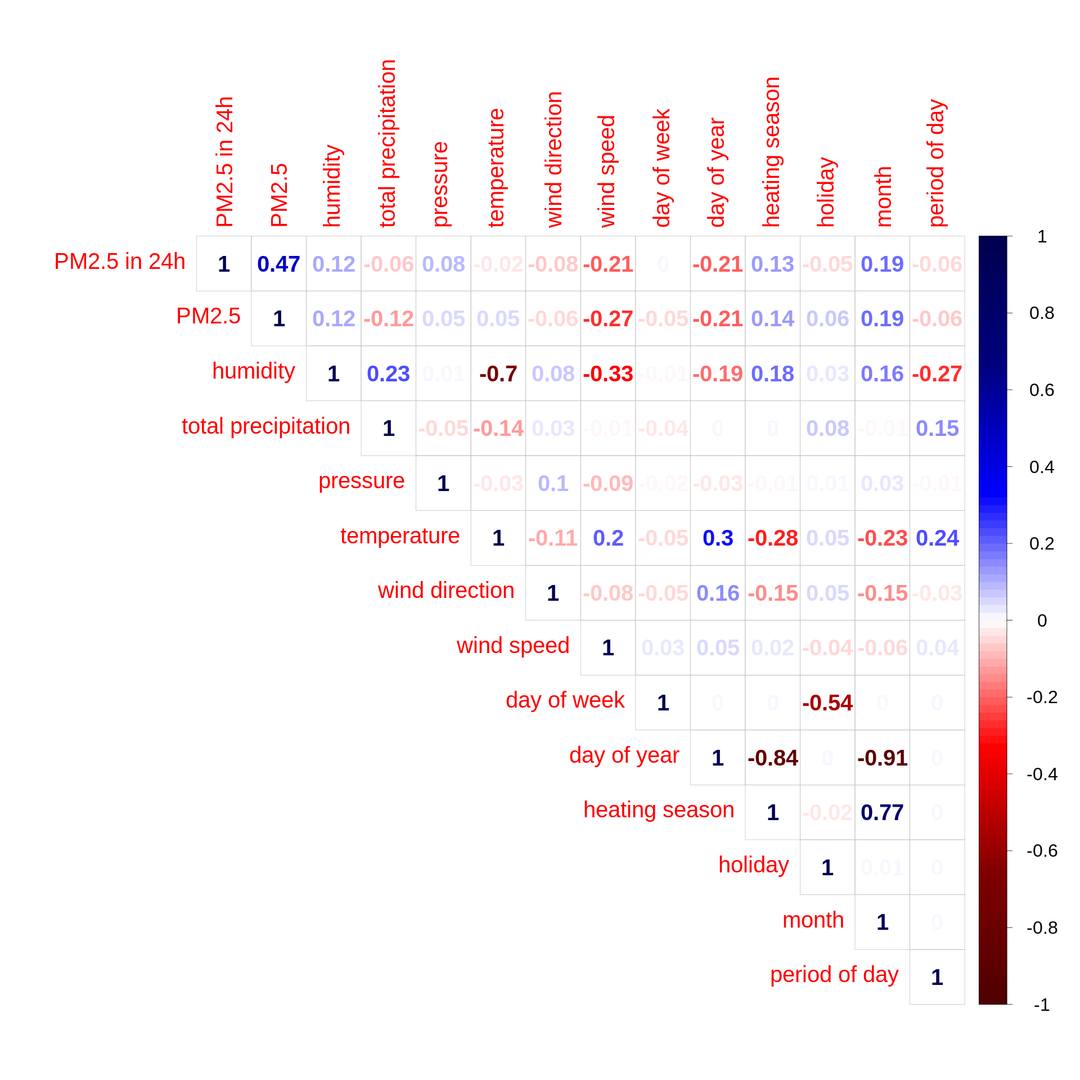
\includegraphics[width=\linewidth]{figures/dataset/correlation/corrplot_gios_bujaka_3.png}
%       \caption{Correlation plots - summer, GIOŚ Bujaka}
%       \label{fig:dataset-correlation-summer-bujaka}
% \end{figure}
% \begin{figure}[htp]
% \centering
%       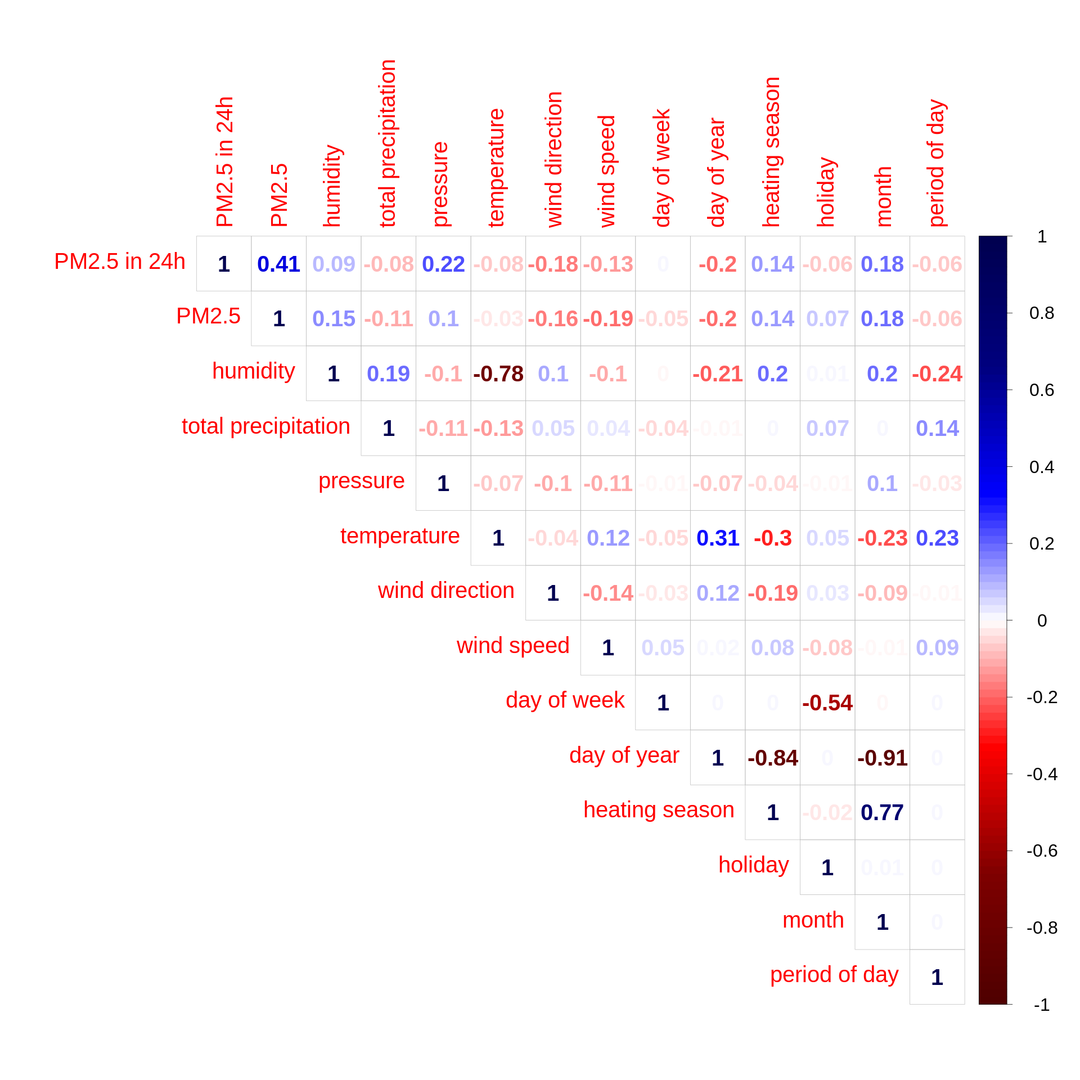
\includegraphics[width=\linewidth]{figures/dataset/correlation/corrplot_gios_bulwarowa_3.png}
%       \caption{Correlation plots - summer, GIOŚ Bulwarowa}
%       \label{fig:dataset-correlation-summer-bulwarowa}
% \end{figure}
% \begin{figure}[htp]
% \centering
%       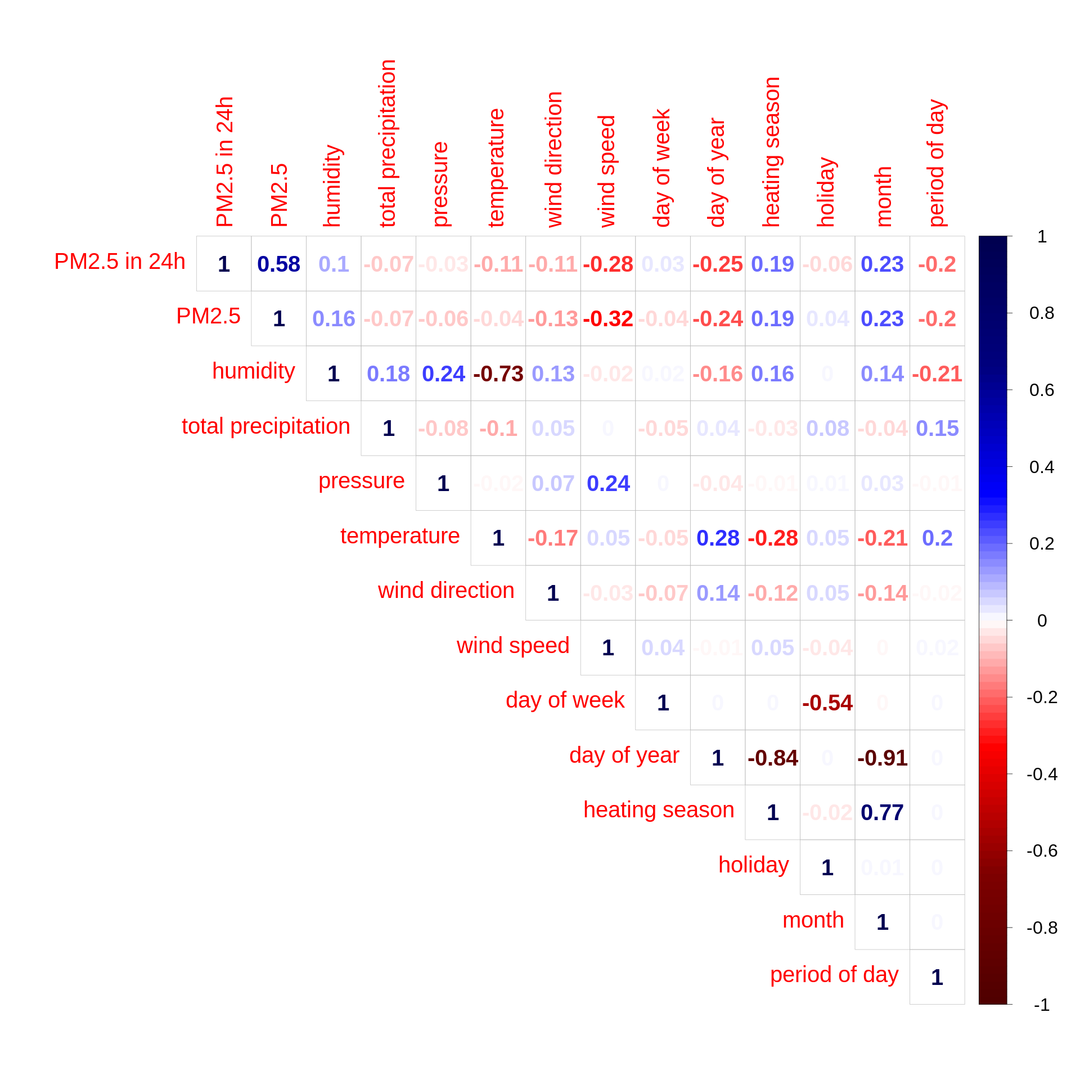
\includegraphics[width=\linewidth]{figures/dataset/correlation/corrplot_gios_krasinskiego_3.png}
%       \caption{Correlation plots - summer, GIOŚ Krasińskiego}
%       \label{fig:dataset-correlation-summer-krasinskiego}
% \end{figure}

% \begin{figure}[htp]
% \centering
%       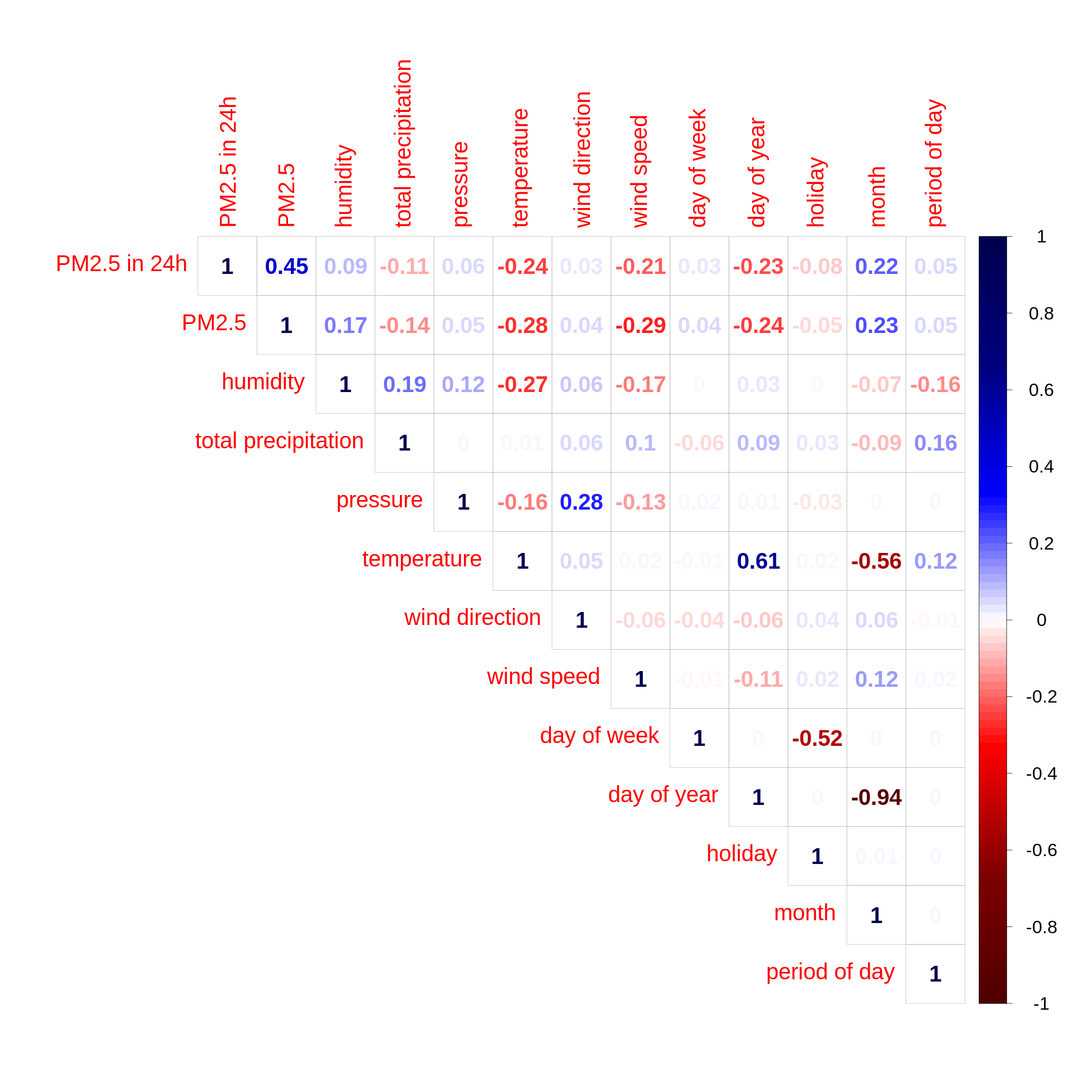
\includegraphics[width=\linewidth]{figures/dataset/correlation/corrplot_gios_bujaka_4.png}
%       \caption{Correlation plots - autumn, GIOŚ Bujaka}
%       \label{fig:dataset-correlation-autumn-bujaka}
% \end{figure}
% \begin{figure}[htp]
% \centering
%       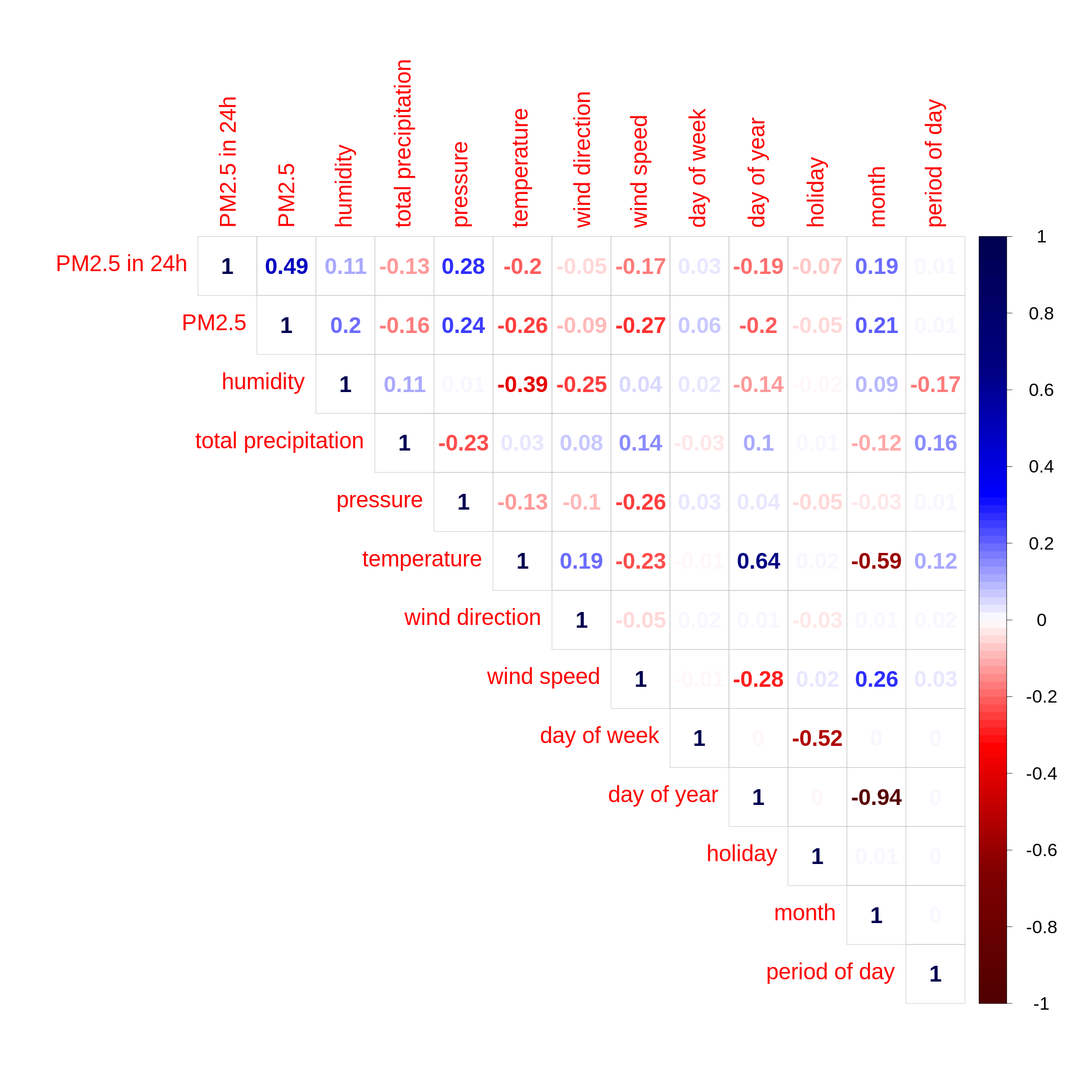
\includegraphics[width=\linewidth]{figures/dataset/correlation/corrplot_gios_bulwarowa_4.png}
%       \caption{Correlation plots - autumn, GIOŚ Bulwarowa}
%       \label{fig:dataset-correlation-autumn-bulwarowa}
% \end{figure}
% \begin{figure}[htp]
% \centering
%       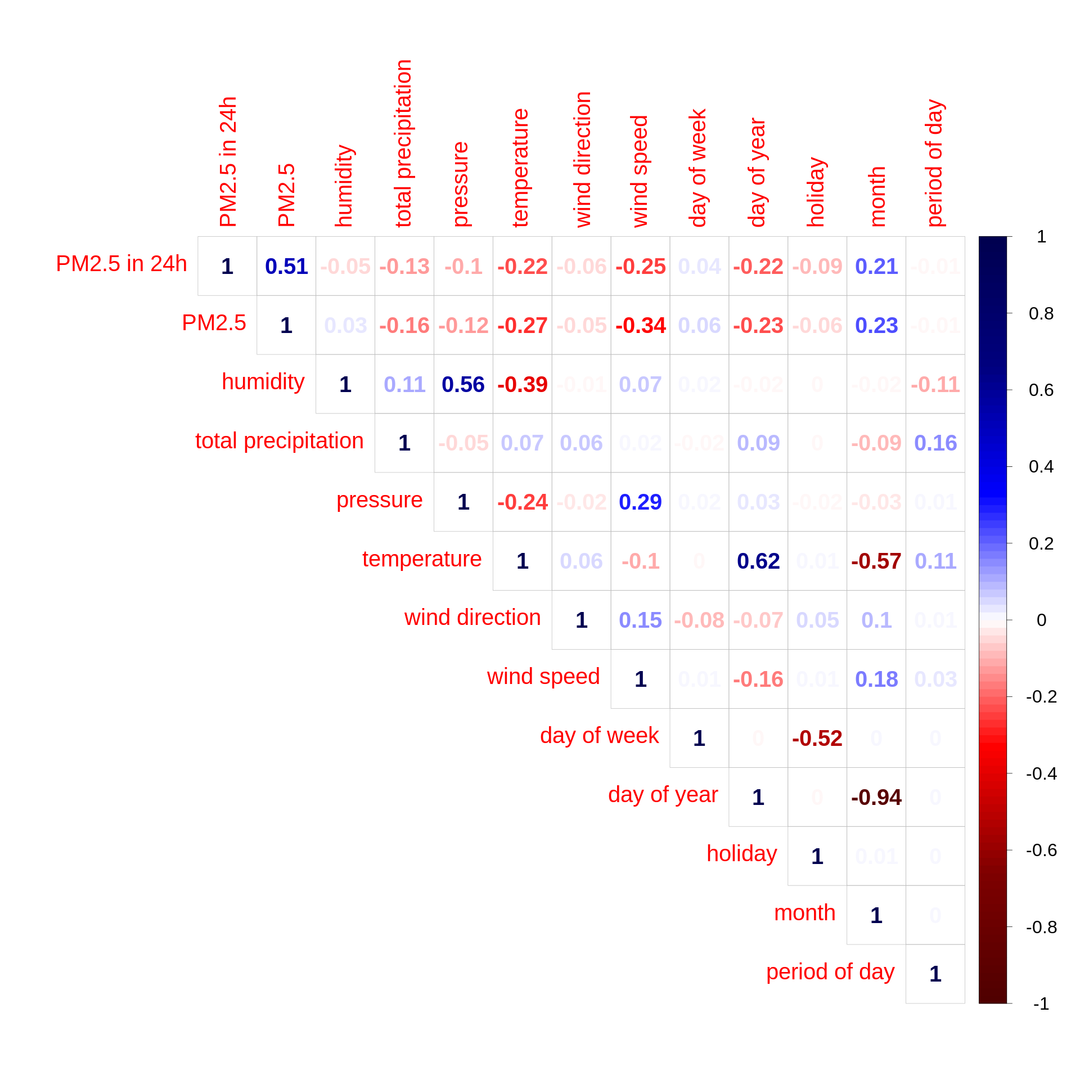
\includegraphics[width=\linewidth]{figures/dataset/correlation/corrplot_gios_krasinskiego_4.png}
%       \caption{Correlation plots - autumn, GIOŚ Krasińskiego}
%       \label{fig:dataset-correlation-autumn-krasinskiego}
% \end{figure}


\begin{landscape}
\begin{table}[H]
\centering
\footnotesize
\caption{Variables with absolute correlation to future PM2.5 concentrations greater than 0.2}
\label{tab:dataset-correlation-significant}
\begin{tabular}{llrrrrrr}
\toprule
Station & Season & \multicolumn{6}{c}{Significant variables} \\ \midrule
 &  & PM2.5 & temperature & wind speed &  &  &  \\
GIOS Bujaka & winter & 0.438 & -0.374 & -0.333 &  &  &  \\ \midrule
 &  & PM2.5 & temperature & pressure & wind speed &  &  \\
GIOS Bulwarowa & winter & 0.429 & -0.336 & 0.249 & -0.249 &  &  \\ \midrule
 &  & PM2.5 & temperature & pressure & wind speed &  &  \\
GIOS Krasinskiego & winter & 0.534 & -0.397 & 0.23 & -0.211 &  &  \\ \midrule
 &  & PM2.5 & day of year & month & heating season & temperature &  \\
GIOS Bujaka & spring & 0.512 & -0.394 & -0.365 & 0.351 & -0.349 &  \\ \midrule
 &  & PM2.5 & day of year & month & temperature & heating season &  \\
GIOS Bulwarowa & spring & 0.497 & -0.404 & -0.379 & -0.351 & 0.316 &  \\ \midrule
 &  & PM2.5 & day of year & temperature & month & heating season & period of day \\
GIOS Krasinskiego & spring & 0.542 & -0.393 & -0.376 & -0.37 & 0.282 & -0.223 \\ \midrule
 &  & PM2.5 & wind speed & day of year &  &  &  \\
GIOS Bujaka & summer & 0.462 & -0.223 & -0.219 &  &  &  \\ \midrule
 &  & PM2.5 & pressure &  &  &  &  \\
GIOS Bulwarowa & summer & 0.411 & 0.228 &  &  &  &  \\ \midrule
 &  & PM2.5 & wind speed & day of year & month &  &  \\
GIOS Krasinskiego & summer & 0.556 & -0.276 & -0.236 & 0.217 &  &  \\ \midrule
 &  & PM2.5 & temperature & day of year & month & wind speed &  \\
GIOS Bujaka & autumn & 0.446 & -0.237 & -0.223 & 0.214 & -0.204 &  \\ \bottomrule
 &  & PM2.5 & pressure & month &  &  &  \\
GIOS Bulwarowa & autumn & 0.442 & 0.257 & 0.203 &  &  &  \\ \midrule
 &  & PM2.5 & wind speed & temperature & day of year & month &  \\
GIOS Krasinskiego & autumn & 0.502 & -0.246 & -0.222 & -0.21 & 0.204 &  \\ \midrule
\end{tabular}
\end{table}
\end{landscape}